\documentclass[a4paper,10pt,openany]{book}
\usepackage[utf8]{inputenc}
\usepackage[english]{babel}
\usepackage{amsmath,amsthm,amssymb}
\usepackage{array}
\usepackage{mathtools,trimclip,stackengine,scalerel,esvect}
\usepackage[skins]{tcolorbox}
\usepackage{float}
\usepackage{caption}
\usepackage{subcaption}
\usepackage{algorithm}
\usepackage{algorithmic}
\usepackage{enumitem}
\usepackage[colorinlistoftodos,prependcaption]{todonotes}
\usepackage{cite}
\usepackage{tocbibind}
\usepackage[colorlinks,bookmarks=true,bookmarksdepth=2,linkcolor=blue,urlcolor=blue,citecolor=blue]{hyperref}
\usepackage{bookmark}
\usepackage{dsfont}
\usepackage{listings}

\usepackage{accents}
\newcommand{\hvv}[1]{\accentset{\rightharpoonup}{#1}}

\renewcommand{\O}[1]{\ensuremath{\mathcal{O}\left(#1\right)}}
\newcommand\smallO{
  \mathchoice
    {{\scriptstyle\mathcal{O}}}% \displaystyle
    {{\scriptstyle\mathcal{O}}}% \textstyle
    {{\scriptscriptstyle\mathcal{O}}}% \scriptstyle
    {\scalebox{.7}{$\scriptscriptstyle\mathcal{O}$}}%\scriptscriptstyle
  }
\renewcommand{\o}[1]{\ensuremath{\smallO\left(#1\right)}}
\newcommand{\Id}{\ensuremath{\mathds{1}}}
\newcommand{\somme}[2]{\ensuremath{\underset{#1}{\overset{#2}{\sum}}}}
\newcommand{\cross}{\ensuremath{\times}}
\newcommand{\dd}[2]{\ensuremath{\frac{\partial #1}{\partial #2}}}
\newcommand{\ddd}[3]{\ensuremath{\frac{\partial^{#1} #2}{\partial #3^{#1}}}}
\newcommand{\reel}{\ensuremath{\mathds{R}}}
\renewcommand{\vec}{\ensuremath{\boldsymbol}}
\newcommand{\mat}{\ensuremath{\underline}}
\newcommand{\rchapter}[1]{\chapter{#1}\label{chapter::#1}}

% \newsavebox\tmpbox
% \newcommand\hvv[1]{\ThisStyle{%
%   \setbox0=\hbox{$\SavedStyle#1$}
%   \setbox2=\hbox{$%
%     \clipbox{0pt{} \dimexpr\ht0+2.2\LMpt{} 0pt -1pt}{%
%       $\SavedStyle\vv{\phantom{\SavedStyle #1}}$}$}
%     \ensurestackMath{\stackengine{1.7\LMpt}{\SavedStyle#1}{\copy2}{O}{c}{F}{F}{S}}
% }}

\newcommand{\grad}{\ensuremath{\hvv{\nabla}}}

\definecolor{backcolour}{rgb}{0.95,0.95,0.92}
\definecolor{mygreen}{RGB}{0, 153, 0}

\lstdefinestyle{bashStyle}{
    backgroundcolor=\color{backcolour},
    basicstyle=\footnotesize,
    breakatwhitespace=true,
    breaklines=true,
    captionpos=b,
    keepspaces=true,
    showspaces=false,
    showstringspaces=false,
    showtabs=false,
    tabsize=2
}

\lstdefinestyle{pythonStyle}{
    backgroundcolor=\color{backcolour},
    stringstyle=\color{mygreen},
    commentstyle=\color{red},
    basicstyle=\footnotesize,
    breakatwhitespace=true,
    breaklines=true,
    captionpos=b,
    keepspaces=true,
    showspaces=false,
    showstringspaces=false,
    showtabs=false,
    tabsize=2
}


%%%%%%%%%%%%%%%%%%%%%%%%%%%%%%%%%%%%%%%%%%%%%%%%%%%%%%%%%%%%%%%%%%%%%%%%%%%%%%%%%%%%%%%%%%%

% page clearing
\newcommand{\clearemptydoublepage}{%
  \ifthenelse{\boolean{@twoside}}{\newpage{\pagestyle{empty}\cleardoublepage}}%
  {\clearpage}}

%%%%%%%%%%%%%%%%%%%%%%%%%%%%%%%%%%%%%%%%%%%%%%%%%%%%%%%%%%%%%%%%%%%%%%%%%%%%%%%%%%%%%%%%%%%
  
  
\floatstyle{ruled}
\newfloat{Example}{tbp}{lop}[chapter]

% !TEX root = ../main.tex
% Set here the title, authors and other stuff to be used for the cover
% This file is used by MAIN.TEX

% set title, authors and stuff for the cover
\def\university{Technische Universit{\"a}t M{\"u}nchen}
\def\universityLogo{styles/tum_logo}
\def\program{Computational Science and Engineering \\(International Master's Program)}
\def\programLogo{styles/cse_logo}
\def\doctype{Master's Thesis}

\def\title{Parallel gyrokinetic simulations with Python}
\def\titlegerman{Parallele gyrokinetische Simulationen mit Python}
\def\author{Emily Bourne}
\def\examinerOne{Univ.-Prof.\ Dr.\ Eric Sonnendr\"ucker}
\def\assistantAdvisor{Dr.\ rer.\ nat.\ Yaman G\"u\c{c}l\"u}
\def\date{28th September, 2018}

\def\keywords{{gyrokinetics}, {pyccel}, {keyword3}}

% The following are used for the PDF metadata, by default the same as above.
\def\metaTitle{\title}
\def\metaAuthor{\author}
\def\metaSubject{\doctype\ -\ \university}
\def\metaKeywords{\keywords}

% text to appear in the footer
\def\footertext{}


\begin{document}

\frontmatter 

% !TEX root = ../main.tex
% The front cover.
% Included by MAIN.TEX

%--------------------------------------------------
% The Front Cover
%--------------------------------------------------

% correct BCOR - undo at the end !!!
\def\bcorcor{0.15cm}
\addtolength{\hoffset}{\bcorcor}

\thispagestyle{empty}

\vspace{4cm}
\begin{center}
	\includegraphics[width=4cm]{\universityLogo}\\
	\vspace{5mm}
	\huge \program \\
	\vspace{0.5cm}
	\large \university
\end{center}

\vspace{20mm}
\begin{center}
	{\Large \doctype}\\
	\vspace{20mm}
	{\huge \textbf \title}\\
	\vspace{15mm}
	{\LARGE  \author}\\
	\vspace{\fill}
	\includegraphics[width=4cm]{\programLogo}
\end{center}



\clearemptydoublepage

% !TEX root = ../main.tex
% The titlepage.
% Included by MAIN.TEX


%--------------------------------------------------
% The title page
%--------------------------------------------------

% correct BCOR - undo at the end !!!
\def\bcorcor{0.15cm}
\addtolength{\hoffset}{\bcorcor}

\thispagestyle{empty}

\vspace{4cm}
\begin{center}
    \includegraphics[width=4cm]{\universityLogo}\\
    \vspace{5mm}
    \huge \program \\
    \vspace{0.5cm}
    \large \university
\end{center}

\vspace{10mm}
\begin{center}
    {\Large \doctype}\\
    \vspace{10mm}
    {\LARGE \title}\\
    \vspace{10mm}
    {\LARGE \titlegerman}\\
    \vspace{10mm}

    \begin{tabular}{ll}
      \Large Author:                        & \Large \author \\[2mm]
      \Large 1\textsuperscript{st} examiner:& \Large \examinerOne\\[2mm]
      \Large Assistant advisor:             & \Large \assistantAdvisor \\[2mm]
      \Large Submission Date:               & \Large \date
    \end{tabular}

    \vspace{\fill}
    \includegraphics[width=4cm]{\programLogo}
\end{center}

% undo BCOR correction
\addtolength{\hoffset}{\bcorcor}


% !TEX root = ../main.tex
\clearemptydoublepage

\thispagestyle{empty}
\vspace*{0.8\textheight}
\noindent
I hereby declare that this thesis is entirely the result of my own work except where otherwise indicated. I have only used the resources given in the list of references.

\vspace{15mm}
\noindent
\date \hspace{5cm} \author
\newpage


%% !TEX root = ../main.tex
\clearemptydoublepage
\phantomsection
\addcontentsline{toc}{chapter}{Acknowledgements}

\vspace*{2cm}

\begin{center}
{\Large \textbf Acknowledgments}
\end{center}

\vspace{1cm}

\begin{center}
If someone helped you or supported you through your studies, this page is a
good place to tell them how thankful you are.
\end{center}


% !TEX root = ../main.tex
% The abstract.
% Included by MAIN.TEX

\clearemptydoublepage
\phantomsection
\addcontentsline{toc}{chapter}{Abstract}

\vspace*{2cm}
\begin{center}
{\Large \textbf Abstract}
\end{center}
\vspace{1cm}

Pyccel, a python to human-readable Fortran translator, is used to test the feasibility of writing large parallel simulations in python without significant loss of runtime speed as compared to writing in Fortran directly. A parallel simulation of a plasma using gyrokinetic theory is written for this purpose. The simulation uses a field-aligned semi-lagrangian method. Cylindrical (screw-pinch) geometry is used to approximate the shape of the domain. The acceleration obtained using Pyccel is very large. Although the speed of the pure Fortran version is not quite reached, the decrease in the amount of development time required largely offsets this small loss.


\tableofcontents
%e.g. preface

\mainmatter

\rchapter{Introduction}

As an interpreted language, Python runs significantly slower than other languages such as C or Fortran. However, code can usually be developed much faster in Python. As a result, it is preferred by many developers for smaller projects. Although the resulting program runs slower, the trade-off is acceptable as the overall time spent on the project is lower.

The situation is more problematic for large projects. In this case, the runtime can be several days. A program written in Python often runs as much as 100 times slower than its equivalent in C or Fortran. This would therefore lead to a runtime of close to one year. This is especially problematic as the simplicity of Python means that many scientists rarely use lower level languages and are thus out of practice when they need to use them.

Multiple solutions exist to try and improve this situation which consists of accelerating Python code so that it runs at speeds which more closely approach those seen in C or Fortran. One type of solution is just-in-time compilers such as PyPy and numba. Pypy is especially powerful as it requires no changes to the code. It can thus adapt the function to the types that are used when it is called, however many packages are not supported and the entire code must be run using pypy. In contrast, numba does not need to be used everywhere, but cannot be used immediately. It requires the types used by the function to be declared in a decorator. This however, means that it can reuse the compiled code making it faster when calls are reused a lot.

Another alternative is to use ahead-of-time compilers such as cython or pythran. Numba also has an ahead-of-time compiler. These tools can be more cumbersome. The type of the arguments must always be given, however they can potentially lead to large speed-ups when used. These tools each work in different ways, for example numba requires only a decorator added to the function which will be compiled. It then compiles the code directly and generates a shared object file. In contrast cython translates the code to C which can then be compiled and called from Python. The advantage of generating code in another language is that it can be compiled with different compilers. It is also possible to modify the resulting code if there are improvements possible which cannot be mimicked in Python. Unfortunately the code generated by cython is rarely human readable so this second advantage is lost.

In this project another ahead-of-time compiler will be used: pyccel. Like cython, Pyccel translates the Python code into another language, in this case Fortran. However, unlike for cython, the code generated by pyccel is human-readable. It is also simple to use, requiring only that a decorator be added to the functions to be translated. Its simplicity, the scale of the speed-up that can be achieved, and the fact that the generated code can be modified to give improve the functions further when required, make pyccel a very useful tool for rapidly developing projects.

The magnitude of the difference in speed between Python and C or Fortran is however so large that it is important to examine the effect that pyccel can have on all aspects of the development of a project in order to determine whether the speed-up achieved is sufficient to allow the development of scientific code in Python. In this project a gyrokinetic plasma simulation is developed in Python. It is then accelerated using pyccel and the resulting program is compared with a Fortran version of the same simulation.

The simulation which will be explored was first developed by Latu et al. \cite{YamanPaper} in their paper Field-Aligned Interpolation for Semi-Lagrangian Gyrokinetic Simulations. In plasma simulations, many points are needed in order to accurately represent all of phase space. This is very costly. As a result many methods have been developed allowing the number of points needed, to be reduced. Gyrokinetic theory allows the problem to be reduced from six dimensions to five (or four for collisionless models). The field-aligned interpolation method explored in the paper by Latu et al. allows fewer points to be used along the toroidal axis



\rchapter{Gyrokinetics}

\section{Introduction}

Particles in a plasma follow a complicated movement determined by electric and magnetic fields. The combination of the fields makes the particles move in a spiral motion around a guiding centre as shown by figure \ref{fig::guiding centre}.

\begin{figure}[ht]
 \centering
 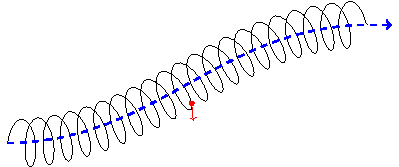
\includegraphics[width=.8\textwidth]{Figs/GyrokineticPrinciple}
 \caption{\label{fig::guiding centre}Path of a particle in a magnetic field and the guiding centre of that particle (shown in dashed blue)}
\end{figure}

This gyro-rotation is problematic for simulations as this motion means that the phase-space coordinates of the particle change rapidly. As a result, small time steps are required to obtain an accurate solution. Fortunately the high frequency gyro-rotation does not have an important effect on the low frequency physics demonstrated by the plasma, as a result if this motion can be rigorously removed from the equations of motion then the resulting equations which are less constrained can be used to analyse low frequency behaviour. In addition, the removal of this high frequency motion allows the reduction of the 6-D problem to a 5-D problem. This is the aim of gyrokinetics.

There are multiple methods used for finding the equations used in gyrokinetics (for example as described by Sugama et al \cite{Sugama2000}, Brizard \cite{BrizardGyro2000}, and others) which include some kind of coordinate transformations. The result of these transformations is that the coordinates are $(\vec{x},v_\parallel,\mu)$ where $\vec{x}$ is the position of the gyro centre, $v_\parallel$ is the velocity parallel to the time-independent background magnetic field $B_0$, and $\mu$ is the conserved magnetic moment. Normally there would also be a coordinate $\theta$ representing the gyroangle which is necessary to handle time-dependent fluctuations in the magnetic field, however the gyrokinetic transformations move these dependencies so that they are averaged which then removes them from the final equations. As a result the problem is reduced to five dimensions.

\section{Continuity Equation}

In the simulations, the plasma is described by a distribution function. This function describes the positions of a collection of identical particles of charge $q\neq 0$ and mass $m > 0$, immersed in a static magnetic field B(x). This value of this function is therefore conserved along particle trajectories\cite{MonteCarloBottino}:

\begin{equation}
 f\left(\vec{Z}\left(\vec{Z}_0,t\right),t\right) = f\left(\vec{Z}_0,t_0\right)
\end{equation}

The corresponding conservation equation is therefore defined as follows:

\begin{equation}
 \frac{d}{dt} f\left(\vec{Z}\left(\vec{Z}_0,t\right),t\right) = \dd{}{t}f\left(\vec{Z},t\right) + \underset{\alpha}{\sum} \frac{d\vec{Z}_\alpha}{dt}\dd{}{\vec{Z}}f\left(\vec{Z},t\right) = 0
\end{equation}

For the gyro-centre distribution function which is used for gyrokinetic theory, $f\in\reel_+$ and is a function of time $t\in\reel_+$ and of the phase space coordinates $\left(\vec{x},v_\parallel,\mu\right)$. This yields the following function:

\begin{equation}\label{eq::conservation general}
 \dd{}{t}f + \dot{\vec{x}}\cdot\grad f + \dot{v}_\parallel \dd{f}{v_\parallel} + \dot{\mu} \dd{f}{\mu} = 0
\end{equation}

The values of $\vec{u}=\dot{\vec{x}}$, $a_\parallel=\dot{v}_\parallel$, $M=\dot{\mu}$ can be determined using the Euler-Lagrange equations:

\begin{equation}
 \frac{d}{dt}\left(\dd{\mathcal{L}}{\dot{\vec{Z}}_\alpha}\right)-\dd{\mathcal{L}}{\vec{Z}_\alpha}=0
\end{equation}

where $\mathcal{L}$ is the Lie-transformed low-frequency particle Lagrangian obtained using gyrokinetic theory, defined (in SI units) as follows \cite{MonteCarloBottino}:

\begin{equation}
 L=\left(e\vec{A}+mv_\parallel\hat{b}\right)\cdot\dot{\vec{x}}+\frac{m\sqrt{4\pi}}{e\mu_0^{\frac{3}{2}}}\mu\dot{\theta}-H\left(\vec{x},v_\parallel\right)
\end{equation}

Although $\theta$ is not one of the gyrokinetic coordinates, it is a phase-space coordinate and as such can also be used to obtain useful equations. The Euler-Lagrange equation for $\theta$ is as follows:
\begin{align}
 \frac{d}{dt}\left(\frac{m\sqrt{4\pi}}{e\mu_0^{\frac{3}{2}}} \mu\right) + 0 = 0\\
 \dot{\mu} = 0\label{eq::mu dot def}
\end{align}

This implies that $M=\dot{\mu}=0$.

The Euler-Lagrange equation for $v_\parallel$ is as follows:

\begin{align}
 \frac{d}{dt}\Big(0\Big) - m \hat{b}\cdot\dot{\vec{x}}+\dd{H}{v_\parallel}=0\\
 \hat{b}\cdot\dot{\vec{x}}=\frac{1}{m}\dd{H}{v_\parallel}\label{eq::bxdotDefinition}
\end{align}

The Euler-Lagrange equation for $\vec{x}$ is as follows:

\begin{align}
 \frac{d}{dt}\left(e\vec{A}+mv_\parallel\hat{b}\right) - e\grad\left(A\cdot\dot{\vec{x}}\right)-mv_\parallel\grad\left(\hat{b}\cdot\dot{\vec{x}}\right) + \grad H = 0\\
 e\mathcal{J}_{\vec{A}}\dot{\vec{x}} + ma_\parallel\hat{b} + mv_\parallel\mathcal{J}_{\hat{b}}\dot{\vec{x}} - e\mathcal{J}_{\vec{A}}^T\dot{\vec{x}} - mv_\parallel\mathcal{J}_{\hat{b}}^T\dot{\vec{x}} + \grad H = 0\\
 \dot{v_\parallel}\hat{b} = \frac{e}{m}\left(\mathcal{J}_{\vec{A}}^T-\mathcal{J}_{\vec{A}}\right)\dot{\vec{x}} + v_\parallel \left(\mathcal{J}_{\hat{b}}^T-\mathcal{J}_{\hat{b}}\right)\dot{\vec{x}} - \frac{1}{m}\grad H
\end{align}

We now simplify the equations by introducing the following definitions:

\begin{gather}
 \vec{A}^*=\vec{A}+\frac{mv_\parallel}{e}\hat{b}\\
 \vec{B}^*=\grad\cross\vec{A}^* = \vec{B}+\frac{mv_\parallel}{e}\grad\cross\hat{b}
\end{gather}

Which leaves us with the equation:

\begin{align}\label{eq::EulerLagX}
 \dot{v_\parallel}\hat{b} = \frac{e}{m}\left(\mathcal{J}_{\vec{A}^*}^T-\mathcal{J}_{\vec{A}^*}\right)\dot{\vec{x}} - \frac{1}{m}\grad H
\end{align}

This equation can be simplified by remarking that $\left({\mathcal{J}_A^T}-{\mathcal{J}_A}\right)\vec{C} = \vec{C}\cross\left(\grad\cross\vec{A}\right)$ for all vector $\vec{C}$:

\begin{align*}
 \left[\vec{C}\cross\left(\grad\cross\vec{A}\right)\right]_i &= \varepsilon_{ijk}c_j\varepsilon_{klm}\partial_la_m\\
 &= \varepsilon_{kij}\varepsilon_{klm}c_j\partial_la_m\\
 &= \left(\delta_{il}\delta_{jm}-\delta_{im}\delta_{jl}\right)c_j\partial_la_m\\
 &= c_j\partial_ia_j - c_j\partial_ja_i\\
 &=\left({\mathcal{J}_A^T}_{ij}-{\mathcal{J}_A}_{ij}\right)c_j\\
 &=\left[\left({\mathcal{J}_A^T}-{\mathcal{J}_A}\right)\vec{C}\right]_i
\end{align*}

Equation \ref{eq::EulerLagX} is then written as follows:

\begin{align}
 \dot{v_\parallel}\hat{b} &= \frac{e}{m}\dot{\vec{x}}\cross\left(\grad\cross\vec{A}^*\right) - \frac{1}{m}\grad H\\
  &= \frac{e}{m}\dot{\vec{x}}\cross\vec{B}^* - \frac{1}{m}\grad H\label{eq::vbDefinition}
\end{align}

This expression can now be used to find a definition of $a_\parallel = \dot{v_\parallel}$. This is done by taking the dot product of the equation and $\hat{b}$:

\begin{align}
 \dot{v_\parallel}\vec{B}^*\cdot\hat{b} &= \frac{e}{m}\vec{B}^*\cdot\left(\dot{\vec{x}}\cross\vec{B}^*\right) - \frac{1}{m}\vec{B}^*\cdot\grad H\\
 \dot{v_\parallel} &= - \frac{\vec{B}^*}{mB_\parallel^*}\cdot\grad H\label{eq::a_parallel def}
\end{align}

where $B_\parallel^*=\hat{b}\cdot\vec{B}^*$.

The definition of $\vec{u}=\dot{\vec{x}}$ can also be found from equations \ref{eq::bxdotDefinition} and \ref{eq::vbDefinition} by taking the cross product of equation \ref{eq::vbDefinition} and $\hat{b}$ :

\begin{align}
 \dot{v_\parallel} \hat{b}\cross\hat{b} &= \frac{e}{m}\hat{b}\cross\left(\dot{\vec{x}}\cross\vec{B}^*\right) - \frac{1}{m}\hat{b}\cross\grad H\\
 0 &= \frac{e}{m}\left(\left(\hat{b}\cdot\vec{B}^*\right)\dot{\vec{x}}-\left(\hat{b}\cdot\dot{\vec{x}}\right)\vec{B}^*\right) - \frac{1}{m}\hat{b}\cross\grad H\\
 \frac{eB_\parallel^*}{m}\dot{\vec{x}} &= \frac{e}{m^2}\dd{H}{v_\parallel}\vec{B}^* + \frac{1}{m}\hat{b}\cross\grad H\\
 \dot{\vec{x}} &= \frac{1}{mB_\parallel^*}\dd{H}{v_\parallel}\vec{B}^* + \frac{1}{eB_\parallel^*} \hat{b}\cross\grad H\label{eq::u def}
\end{align}

The equations obtained using the Euler Lagrange equations (equations \ref{eq::mu dot def} \ref{eq::a_parallel def} \ref{eq::u def}) can now be substituted into equation \ref{eq::conservation general} to define the problem:

\begin{gather}
 \dd{}{t}f + \vec{u}\cdot\grad f + a_\parallel \dd{f}{v_\parallel} + \vec{M} \dd{f}{\mu} = 0\\
 \vec{u} = \frac{1}{mB_\parallel^*}\dd{H}{v_\parallel}\vec{B}^* + \frac{1}{eB_\parallel^*} \hat{b}\cross\grad H\\
 a_\parallel = - \frac{\vec{B}^*}{mB_\parallel^*}\cdot\grad H\\
 \vec{M}=0
\end{gather}

This expression depends on the Hamiltonian of the system which is defined using gyrokinetic theory as follows (in SI units) \cite{YamanPaper}: 

\begin{equation}
 H=\frac{1}{2}mv_\parallel^2 + \mu B(\vec{x})+e\langle\phi\rangle_g(t,\vec{x})
\end{equation}

This leaves the following definitions for the advection coefficients:

\begin{align}
 \vec{u} =& \frac{v_\parallel\vec{B}^*}{B_\parallel^*} + \frac{1}{eB_\parallel^*} \hat{b}\cross\left(\mu\grad B(\vec{x})+e\grad\phi\right) \label{eq::General u}\\
 a_\parallel =& - \frac{\vec{B}^*}{mB_\parallel^*}\cdot\left(\mu\grad B(\vec{x})+e\grad\phi\right)\label{eq::General a parallel}
\end{align}

\subsection{Cylindrical Geometry}

Generally the definition of the magnetic field used will be that used by Latu et al \cite{YamanPaper}:

\begin{align}
 \vec{B}=&\frac{B_0R_0}{R}\left(\zeta(r)\hat{\theta}+\hat{\varphi}\right) &&
 \zeta(r)=\frac{r}{q(r)R_0}
\end{align}

where $R_0$ is the major radius, $B_0$ is the toroidal magnetic field at the magnetic axis, $R(r,\theta) = R_\theta + r \cos\theta$ , and $q(r)$ is the classical safety factor in the large aspect ratio limit ($\frac{r}{R_0}\rightarrow 0$).

In the simplified case of a straight periodic cylinder, the toroidal angular variable $\hat{\varphi}$ is replaced by a straight variable $\hat{z} = R_0 \hat{\varphi}$, and R is taken to be equal to $R_0$. This leaves the following expression for the magnetic field:

\begin{align}
 \vec{B}=&B_0\left(\zeta(r)\hat{\theta}+\hat{z}\right) && \zeta(r)=\frac{\iota(r)r}{R_0}
\end{align}

where $\iota(r)=\frac{1}{q(r)}$.

The unit vector $\hat{b}$ is therefore defined as follows:

\begin{equation}\label{eq::magnetic unit}
\hat{b}=
\begin{cases}
 b_r=0\\
 b_\theta=\frac{s\zeta}{\sqrt{1+\zeta^2}}\\
 b_z=\frac{s}{\sqrt{1+\zeta^2}}
\end{cases}
\end{equation}

where $s=\text{sgn}(B_0)$.

This formulation has the advantage of simplifying equations \ref{eq::General u} and \ref{eq::General a parallel} as $\grad B=\vec{0}$. This can be proven using the fact that $B=\|\vec{B}\|$ and that it only depends on $r$. This means that $\left(\grad B\right)_\theta = \left(\grad B\right)_z = 0$ and $\left(\grad B\right)_r$ is determined below:

\begin{align*}
 \left(\grad B\right)_r =& \partial_r \sqrt{\underset{i}{\sum}B_i(r)^2}\\
 =&\frac{1}{B}\underset{i}{\sum} B_i(r) \partial_r B_i(r)\\
 =& \frac{1}{B}\left( B_\theta \partial B_\theta + B_z \partial_r B_z\right)\\
 =& \frac{1}{B}\left( \frac{s\zeta}{(1+\zeta^2)^{\frac{1}{2}}}\frac{s\partial_r\zeta}{(1+\zeta^2)^{\frac{3}{2}}} + \frac{s}{(1+\zeta^2)^{\frac{1}{2}}}\frac{-s\zeta\partial_r\zeta}{(1+\zeta^2)^{\frac{3}{2}}}\right)\\
 =& \frac{1}{B}\left( \frac{\zeta\partial_r\zeta}{(1+\zeta^2)^2}-\frac{\zeta\partial_r\zeta}{(1+\zeta^2)^2}\right)\\
 =& 0
\end{align*}

Equations \ref{eq::General u} and \ref{eq::General a parallel} can therefore be written as follows:

\begin{align}
 \vec{u} =& \frac{v_\parallel\vec{B}^*}{B_\parallel^*} + \frac{1}{B_\parallel^*} \hat{b}\cross\grad\phi\\
 a_\parallel =& - \frac{e\vec{B}^*}{mB_\parallel^*}\cdot\grad\phi
\end{align}

These equations are expressed in the orthogonal basis $(\hat{r},\hat{\theta},\hat{z})$. However for field-aligned expressions we are interested in objects which are parallel to the magnetic field. It is therefore important to identify these objects by including the magnetic unit vector $\hat{b}$ in the equations. In order to do this, the equations will now be expressed on the non-orthogonal basis $(\hat{r},\hat{\theta},\hat{b})$. These expressions can be found using the following definitions for an arbitrary vector $\vec{v}$:

\begin{equation*}
 \vec{v}=v_1\hat{r} + v_2\hat{\theta} + v_3\hat{z} \quad \quad \quad = v_1 \hat{r} + w_1\hat{\theta} + w_2\hat{b}
\end{equation*}
\vspace{-1.5em}
\begin{align*}
 w_1 =& \frac{v_2\hat{b}\cross\hat{\theta} + v_3\hat{b}\cross\hat{z}}{\hat{b}\cross\hat{\theta}}\\
 =& v_2 - v_3 \frac{b_\theta}{b_z}\\
 =& v_2 - v_3 \zeta\\
 w_2 =& \frac{v_3\hat{\theta}\cross\hat{z}}{\hat{\theta}\cross\hat{b}}\\
 =& \frac{v_3}{b_z}
\end{align*}

In order to express $a_\parallel$ in the non-orthogonal coordinates, $\vec{B}^*(x,v_\parallel)$ must first be expressed. In order to express $\vec{B}^*(x,v_\parallel)$, $\grad\cross\hat{b}$ is also needed:
\begin{align*}
 \grad\cross\hat{b} =& -\partial_rb_z\hat{\theta}+\frac{1}{r}\partial_r(rb_\theta)\hat{z}\\
 =& \left(\frac{s\zeta \zeta'}{\left(1+\zeta^2\right)^{\frac{3}{2}}}\right)\hat{\theta} + \left(\frac{s\zeta}{r\left(1+\zeta^2\right)^{\frac{1}{2}}} + \frac{s\zeta'}{\left(1+\zeta^2\right)^{\frac{3}{2}}}\right)\hat{z}\\
 =& \left(\frac{s\zeta \zeta'}{\left(1+\zeta^2\right)^{\frac{3}{2}}} - \frac{s\zeta^2}{r\left(1+\zeta^2\right)^{\frac{1}{2}}} - \frac{s\zeta'\zeta}{\left(1+\zeta^2\right)^{\frac{3}{2}}}\right)\hat{\theta}\\
 &+ \left(\frac{s\zeta}{r\left(1+\zeta^2\right)^{\frac{1}{2}}} + \frac{s\zeta'}{\left(1+\zeta^2\right)^{\frac{3}{2}}}\right)\frac{1}{b_z}\hat{b}\\
 =& - \frac{s\zeta^2}{r\left(1+\zeta^2\right)^{\frac{1}{2}}} \hat{\theta} + \left(\frac{\zeta}{r} + \frac{\zeta'}{1+\zeta^2}\right)\hat{b}
\end{align*}
where $\zeta'=\partial_r\zeta(r)$.

$\vec{B}^*(x,v_\parallel)$ can now be expressed:
\begin{align*}
 \vec{B}^*(x,v_\parallel) =& \vec{B}(x) + \frac{m}{e}v_\parallel \grad \cross \hat{b}(x)\\
 =& |B_0|\sqrt{1+\zeta^2}\hat{b}(x) + \frac{m}{e}v_\parallel \left[\frac{s\zeta\zeta'}{\left(1+\zeta^2\right)^{\frac{3}{2}}}\hat{\theta}\right.\\
 & \left.+ \frac{1}{r}\left(\frac{s\zeta}{\left(1+\zeta^2\right)^{\frac{1}{2}}} + \frac{rs\zeta'}{\left(1+\zeta^2\right)^{\frac{3}{2}}}\right)\hat{z}\right]
\end{align*}
\begin{align*}
 =& |B_0|\sqrt{1+\zeta^2}\hat{b}(x) + \frac{m}{e}v_\parallel \left[- \frac{s\zeta^2}{r\left(1+\zeta^2\right)^{\frac{1}{2}}} \hat{\theta} + \left(\frac{\zeta}{r} + \frac{\zeta'}{1+\zeta^2}\right)\hat{b}\right]\\
 =& - \frac{mv_\parallel}{e}\frac{s\zeta^2}{r\left(1+\zeta^2\right)^{\frac{1}{2}}} \hat{\theta} + \left[|B_0|\sqrt{1+\zeta^2} + \frac{mv_\parallel}{e}\left(\frac{\zeta}{r} + \frac{\zeta'}{1+\zeta^2}\right)\right]\hat{b}
\end{align*}

This leaves the following expression for $a_\parallel$:
\begin{align}
a_\parallel =& - \frac{e\vec{B}^*}{mB_\parallel^*}\cdot\grad\phi\nonumber\\
=& -\frac{e}{mB_\parallel^*}\left[-\frac{mv_\parallel}{e}\frac{s\zeta^2}{r^2\sqrt{1+\zeta^2}}\partial_\theta\phi + \left(|B_0|\sqrt{1+\zeta^2}\right.\right.\nonumber\\
&\left.\left.+\frac{mv_\parallel}{e}\left(\frac{\zeta}{r}+\frac{\zeta'}{1+\zeta^2}\right)\right)\hat{b}\cdot\grad\phi\right]\label{eq::a_parallel def cylinder}
\end{align}

In order to also express $\vec{u}$, $\hat{b}\cross\grad\phi$ must also be expressed:

\begin{align*}
 \hat{b}\cross\grad\phi =& \left(b_\theta \partial_z\phi - b_z \frac{\partial_\theta \phi}{r} \right)\hat{r} + b_z \partial_r\phi \hat{\theta} - b_\theta \partial_r \phi \hat{z}\\
 =& \left(b_\theta \partial_z\phi - b_z \frac{\partial_\theta \phi}{r} \right)\hat{r} + \left(b_z \partial_r\phi + \frac{b_\theta^2}{b_z} \partial_r \phi\right) \hat{\theta} - \frac{b_\theta}{b_z} \partial_r \phi \hat{b}\\
 =& \left[\frac{b_\theta}{b_z}\left(\hat{b}\cdot\grad\phi - b_\theta \frac{\partial_\theta\phi}{r}\right) - b_z \frac{\partial_\theta \phi}{r} \right]\hat{r} + \left(\frac{b_z^2 + b_\theta^2}{b_z} \right)  \partial_r\phi \hat{\theta} - \frac{b_\theta}{b_z} \partial_r \phi \hat{b}\\
 =& \left[\frac{b_\theta}{b_z}\hat{b}\cdot\grad\phi - \frac{1}{b_z} \frac{\partial_\theta \phi}{r} \right]\hat{r} + \frac{1}{b_z}   \partial_r\phi \hat{\theta} - \frac{b_\theta}{b_z} \partial_r \phi \hat{b}\\
\end{align*}

This leaves the following expression for $\vec{u}$:
\begin{align}
\vec{u} =& \frac{v_\parallel\vec{B}^*}{B_\parallel^*} + \frac{1}{B_\parallel^*} \hat{b}\cross\grad\phi\nonumber\\
=& \frac{1}{B_\parallel^*} \left[\left(\zeta\hat{b}\cdot\phi - \frac{s}{\sqrt{1+\zeta^2}}\frac{\partial_\theta\phi}{r}\right)\hat{r} \right.\nonumber\\
&+ \left(\frac{s}{\sqrt{1+\zeta^2}}\partial_r\phi - \frac{mv_\parallel^2}{e}\frac{s\zeta^2}{r\sqrt{1+\zeta^2}}\right)\hat{\theta}\nonumber\\
&+ \left.\left(|B_0|\sqrt{1+\zeta^2}v_\parallel + \frac{mv_\parallel^2}{e}\left(\frac{\zeta}{r} + \zeta'\frac{\zeta^2}{1+\zeta^2}\right)-\zeta \partial_r\phi\right)\hat{b}\right]\label{eq::u def cylinder}
\end{align}

In order to complete the definition, $B^*_\parallel$ is also expressed explicitly:
\begin{align}
 B^*_\parallel =& B^*_\theta b_\theta + B^*_z\nonumber\\
 =& |B_0|\sqrt{1+\zeta^2} + \frac{mv_\parallel}{e}\left(-\frac{\zeta^3}{r\left(1+\zeta^2\right)} + \frac{\zeta}{r} + \frac{\zeta'}{1+\zeta^2}\right)\nonumber \\
 =& |B_0|\sqrt{1+\zeta^2} + \frac{mv_\parallel}{e}\left(\frac{\zeta+\zeta'r}{r\left(1+\zeta^2\right)}\right)\label{eq::B parallel star cylinder}
\end{align}

For a torus to be effectively approximated by a straight cylinder, the major radius must be very large. As a result we let $\zeta(r)$ and $\zeta'(r)$ tend to 0. Applying this condition to equations \ref{eq::a_parallel def cylinder}, \ref{eq::u def cylinder}, and \ref{eq::B parallel star cylinder} gives the following expressions:

\begin{align}
 \vec{u} =& -\frac{1}{B_0}\frac{\partial_\theta\phi}{r} \hat{r} + \frac{1}{B_0}\partial_r\phi\hat{\theta} + v_\parallel \hat{b}\\
 a_\parallel =& -\frac{e}{m}\hat{b}\cdot\grad\phi
\end{align}

Thus equation \ref{eq::conservation general} can be written as follows:

\begin{gather}
 \partial_t f + \left(-\frac{1}{B_0}\frac{\partial_\theta\phi}{r} \hat{r}+\frac{1}{B_0}\partial_r\phi\hat{\theta} + v_\parallel \hat{b}\right)\cdot\grad f -\frac{e}{m}\hat{b}\cdot\grad\phi\,  \partial_{v_\parallel} f=0\\
 \partial_t f -\frac{1}{B_0}\frac{\partial_\theta\phi}{r} \partial_r f + \frac{1}{B_0}\partial_r\phi \frac{\partial_\theta\phi}{r} + v_\parallel \grad_\parallel f - \frac{e}{m}\grad_\parallel\phi\,  \partial_{v_\parallel} f=0
\end{gather}

To simplify the expression a Poisson bracket notation is introduced, defined as follows:
\begin{equation}
 \{\phi,f\}=-\frac{\partial_\theta\phi\partial_rf}{rB_0}+\frac{\partial_r\phi\partial_\theta f}{rB_0}
\end{equation}

This leaves the following final expression:

\begin{equation}\label{eq::Continuity Cylindrical}
 \partial_t f + \{\phi,f\} + v_\parallel \grad_\parallel f - \frac{e}{m}\grad_\parallel\phi\,  \partial_{v_\parallel} f=0
\end{equation}

\section{Quasi-Neutrality Equation}
% 
% Maxwell equations (in SI units):
% 
% \begin{align}
%  \grad \cdot \vec{E} &= \frac{\rho}{\varepsilon_0} &&= \frac{\underset{s}{\sum}q_sn_s}{\varepsilon_0} \label{Gauss Law}\\
%  \grad \cross \vec{E} &= -\frac{\partial \vec{B}}{\partial t}\label{Maxwell Faraday equation}\\
%  \grad \cdot \vec{B} &= 0 \label{Gauss Law Magnetism}\\
%  \grad \cross \vec{B} &= \mu_0 \vec{J} + \mu_0\varepsilon_0\dd{\vec{E}}{t} &&= \mu_0\underset{s}{\sum}j_s + \mu_0\varepsilon_0\frac{\partial \vec{E}}{\partial t}\label{Amperes Law}
% \end{align}
% 
% \begin{gather}
%  \vec{B} = \grad \cross \vec{A}\\
%  \vec{E} = -\grad\phi-\dd{\vec{A}}{t}
% \end{gather}
% 
% The Maxwell-Faraday equation (equation \ref{Maxwell Faraday equation}) and Gauss's law for magnetism (equation \ref{Gauss Law Magnetism}) can therefore be derived directly from the definitions of the potentials and the properties of the gradient and the rotational. The remaining two equations can be expressed as follows (using the fact that $\frac{1}{c^2}=\mu_0\varepsilon_0$):
% 
% \begin{gather}
%  \grad^2\phi + \dd{}{t}\left(\grad\cdot\vec{A}\right) = -\frac{\rho}{\varepsilon_0}\\
%  \left(\grad^2 \vec{A} - \frac{1}{c^2}\ddd{2}{A}{t}\right) - \grad\left(\grad\cdot \vec{A}+ \frac{1}{c^2}\dd{\phi}{t}\right)=-\mu_0\vec{J}
% \end{gather}
% 
% For a solution ($\phi$,$\vec{A}$) of the system any potential ($\phi'$,$\vec{A}'$) such that $\phi'=\phi-\dd{\lambda}{t}$, and $\vec{A}' = \vec{A}+\grad\lambda$ is also a solution. To ensure the unicity of the solution a gauge is chosen. A popular gauge is the Coulomb gauge which states that:
% 
% \begin{equation}
%  \grad\cdot\vec{A}=0
% \end{equation}
% 
% This simplifies the equations further leaving the following:
% 
% \begin{gather}
%  \grad^2\phi = -\frac{\rho}{\varepsilon_0}\\
%  \left(\grad^2 \vec{A} - \frac{1}{c^2}\ddd{2}{A}{t}\right) - \frac{1}{c^2}\dd{\grad\phi}{t}=-\mu_0\vec{J}
% \end{gather}
% 
% \begin{equation}
%  n_s = \int \hat{f}_s\delta([\vec{R}+\rho_s]-\vec{x})\mathcal{J}_s d^6Z
% \end{equation}
% 
% $\hat{f}_s$ is the the guiding-centre distribution defined as:
% 
% \begin{align*}
%  \hat{f}_s=&\bar{f}_s + \{\tilde{S},\bar{f}_s\} + \O{\varepsilon_g^2}\\
% 	  =&\bar{f}_s + \{\tilde{S},f_{M_s}  \} + \O{\varepsilon_g^2}
% \end{align*}
% 
% 
% Poisson bracket in gyro-centre coordinates:
% \begin{align}
%  \{F,G\}\equiv \frac{\Omega_s}{B_0}&\left(\dd{F}{\xi} \dd{G}{\mu}-\dd{F}{\mu}\dd{G}{\xi}\right) \nonumber\\
%   + \frac{B^*}{m_sB_\parallel^*}\cdot&\left(\grad F\dd{G}{u} - \dd{F}{u} \grad G\right) - \frac{c}{q_s B_\parallel^*}\vec{b}\cdot\grad F \cross \grad G
% \end{align}

Tronko et al. \cite{TronkoQuasiNeutrality} state the following (re-written in SI units):
\begin{equation}
 -\underset{sp}{\sum}\int dW \frac{1}{B_\parallel^*}\grad_\perp\cdot\left[ B_\parallel^* f_0 \frac{m}{B^2}\grad_\perp \phi_1\right] = \underset{sp}{\sum} q_s \int dW \mathcal{J}_0^{gc}f_1
\end{equation}

$B_\parallel^*$ is defined in equation \ref{eq::B parallel star cylinder} for cylindrical geometry. As above we take the limit $\zeta(r)\rightarrow0$ which leads $B_\parallel^*$ to converge towards the constant $|B_0|$. Given the dependencies of each element the equation can therefore be rewritten as follows:
\begin{align}
 -\underset{sp}{\sum} \grad_\perp\cdot\left[\left(\int dW f_0\right) \frac{m}{B^2}\grad_\perp \phi_1\right] = \underset{sp}{\sum} q_s \int dW \mathcal{J}_0^{gc}f_1\\
 -\underset{sp}{\sum} \grad_\perp\cdot\left[n_0 \frac{m}{B^2}\grad_\perp \phi_1\right] = \underset{sp}{\sum} q_s n_{1s}
\end{align}

Note that $n_{1s}=n_s-n_0$ and for adiabatic electrons $n_e=n_0 \exp\left(-q_e\frac{\phi-\langle \phi\rangle_r}{\kappa T_e}\right)$. The equation can therefore be written as:
\begin{equation}
 -\grad_\perp\cdot\left[\frac{\rho_{m0}}{B^2}\grad_\perp \phi\right] = q_i (n_i-n_0) + q_e n_0 \left(\exp\left(-q_e\frac{\phi-\langle \phi\rangle_r}{\kappa T_e}\right)-1\right)
\end{equation}
where $\rho_{m0}$ is the equilibrium mass density.

The linearisation of the exponential term leads to the following equation:
\begin{equation}
 -\grad_\perp\cdot\left[\frac{\rho_m}{B^2}\grad_\perp \phi\right] = q_i (n_i-n_0) - q_e^2 n_0 \frac{\phi-\langle \phi\rangle_r}{\kappa T_e}
\end{equation}

Dividing by $\varepsilon_0$ we obtain the following equation:
\begin{align}
 -\grad_\perp\cdot\left[\frac{\rho_{m0}}{\varepsilon_0B^2}\grad_\perp\phi\right] + \frac{q_e^2n_{0}}{\varepsilon_0\kappa T_e}\left[\phi-\langle\phi\rangle_f\right]=\frac{1}{\varepsilon_0}\rho_{c1}\\
 -\grad_\perp\cdot\left[\frac{\rho_{m0}}{\varepsilon_0B^2}\grad_\perp\phi\right] + \frac{1}{\lambda_D^2}\left[\phi-\langle\phi\rangle_f\right]=\frac{1}{\varepsilon_0}\rho_{c1}
\end{align}
where $\rho_{c1}$ is the charge perturbation density due to the ions and $\lambda_D=\sqrt{\frac{\varepsilon_0\kappa T_e}{q_e^2n_0}}$ is the electron Debye length.

In the case of non-adiabatic electrons, the electron contribution would take a similar form to the ionic contribution. This would be written as:
\begin{equation}
 -\grad_\perp\cdot\left[\frac{\rho_{m0}}{\varepsilon_0B^2}\grad_\perp\phi\right] + \frac{1}{\lambda_D^2}\left[\phi-\langle\phi\rangle_f\right]=\frac{1}{\varepsilon_0}\rho_{c1}
\end{equation}

as the electron contribution is absorbed by $\rho_{c1}$. The equation can also be simplified by removing the term $\langle\phi\rangle_f$. The final expression used will therefore be the following:
\begin{equation}\label{eq::quasi neutrality}
 -\grad_\perp\cdot\left[\frac{\rho_{m0}}{\varepsilon_0B^2}\grad_\perp\phi\right]+\frac{1}{\lambda_D^2}\left[\phi-\chi\cdot\langle\phi\rangle_f\right]=\frac{1}{\varepsilon_0}\rho_{c1}
\end{equation}

where $\chi$ is an optional parameter equal to either 0 or 1.

\rchapter{Advection Equations}

\section{Introduction}

Advection equations describe the transport of a conserved quantity. They are therefore necessary to describe the movement of particles in a plasma. The derivation of the advection equations is described in detail in chapter \ref{chapter::Gyrokinetics}.

There are many methods for solving advection equations. In this project a semi-lagrangian method will be used with Strang splitting. 

\section{Semi-Lagrangian Method}

The semi-Lagrangian method is a method of solving advection equations of the form:

\begin{equation}
 \partial_t f(\vec{x},t) + \vec{c}(\vec{x},t) \cdot \grad f(\vec{x},t) = 0
\end{equation}

As described by Garbet et al. \cite{GyrokineticSimulations}, it is a combination of the Eulerian and Lagrangian methods of solving advection equations. The Eulerian method consists of discretising the phase space on a fixed grid, and applying a grid based method such as finite differences, finite volumes, and Fourier transforms. This however leads to restrictions on the time step that can be used due to the CFL condition and can lead to dissipation.

The Lagrangian method takes advantage of the fact that advection equations arise from conservation equations to remove the restrictions on the time step. Conserved quantities are quantities whose values remain constant along a trajectory and thus obey the following rule:

\begin{align}
 &\frac{d}{dt} f(\vec{x}(t),t) &= 0\\
 &\frac{\partial}{\partial t} f(\vec{x}(t),t) + \grad f(x(t),t) \cdot \frac{\partial}{\partial t}\vec{x}(t) &= 0
\end{align}

Evidently this trajectory can therefore be described by the following equation:

\begin{equation}\label{eq::semi lagrangian trajectory definition}
 \frac{\partial}{\partial t}x(t) = c(x,t)
\end{equation}

If this equation can be solved trivially then the exact solution can be easily determined. For example, in the simplified case of a 1-D constant advection problem, the exact solution can be defined as follows:

\begin{equation}
 f(x,t) = f_0(x-ct)
\end{equation}

where $f_0(x)=f(x,0)$.

The Lagrangian method exploits these properties to create a method which does not necessarily have any restrictions on the size of the time step. Indeed the time step has no restrictions if the trajectory can be defined exactly. Otherwise it must be approximated via another method to a sufficient degree of accuracy. The method consists of following specific particles along their trajectories. These particles are chosen using statistical methods. This means that at the beginning of the simulation they should be approximately evenly spaced, however it is not guaranteed that this spacing is maintained. This can lead to areas which at a given time contain very few of the chosen particles. This means that the approximation in that area is not very precise.

The semi-Lagrangian method tries to combine the Eulerian and Lagrangian methods to benefit from the advantages of each. The method is grid-based but still uses trajectory integration. At each time step the trajectory defined by equation \ref{eq::semi lagrangian trajectory definition} is followed back from each grid point to its position at the start of the time step. The value of the function at the starting point is then approximated and the value is saved at the grid point.

There are multiple ways of approximating the value at the grid point. Here splines will be used.

\section{Strang Splitting} \label{sec::Strang}

Advection equations can be expressed as:

\begin{equation}
 \partial_t f = \sum_i L_i(f)
\end{equation}

where $L_i(f)$ is an operator. If the operators can be expressed as matrices then the exact solution can be defined as follows:

\begin{equation}
 f(t) = e^{(\sum_i L_i)t}f_0
\end{equation}

Of course in the case of an advection equation the operator is a derivative not a matrix. However, the definition of the derivative means that it can be represented as a matrix of infinite dimensions. Therefore the approximation is appropriate.

If the matrices are commutative then the solution can be expressed as:

\begin{equation}
 f(t) = \prod_i e^{L_it}f_0
\end{equation}

This means that the numerical equation can be split into multiple equations:

\begin{align}
 f(t) = e^{L_n t} f_{n-1}(t)\\
 f_i(t) = e^{L_i t} f_{i-1}(t)\\
 f_1(t) = e^{L_1 t} f_0
\end{align}

This is useful as the resulting equations are much simpler and can be solved on contiguous data sets.

However the matrices representing the derivatives are not necessarily commutative which means that the equation $e^{A+B}=e^Ae^B$ does not necessarily hold. This means that at each time step there is an error due to this supposition. In the simplest splitting method, Lie splitting, this error is $\o{\tau}$. The Strang splitting method reduces this error to $\o{\tau^2}$. The process is as follows:

\begin{enumerate}
 \item One half time step of the least expensive operators
 \item One time step of the most expensive operator
 \item One half time step of the least expensive operators
\end{enumerate}

The proof of the order of the error is given below, where operators A and B are supposed to be relatively inexpensive compared to operator C:

\begin{align*}
 &e^{A\frac{\tau}{2}}e^{B\frac{\tau}{2}}e^{C\tau}e^{B\frac{\tau}{2}}e^{A\frac{\tau}{2}}\\
 =& \left(\Id + A\frac{\tau}{2} + \frac{A^2\tau^2}{8} + \frac{A^3\tau^3}{48} + \O{\tau^4}\right)\cdot\\
 & \left(\Id + B\frac{\tau}{2} + \frac{B^2\tau^2}{8} + \frac{B^3\tau^3}{48} + \O{\tau^4}\right)\cdot\\
 & \left(\Id + C\tau + \frac{C^2\tau^2}{2} + \frac{C^3\tau^3}{6} + \O{\tau^4}\right)\cdot\\
 & \left(\Id + B\frac{\tau}{2} + \frac{B^2\tau^2}{8} + \frac{B^3\tau^3}{48} + \O{\tau^4}\right)\cdot\\
 & \left(\Id + A\frac{\tau}{2} + \frac{A^2\tau^2}{8} + \frac{A^3\tau^3}{48} + \O{\tau^4}\right)\\
 =& \Id + \left(A+B+C\right)\tau + (A+B+C)^2\frac{\tau^2}{2} + \O{\tau^3}\\
 =& e^{(A+B+C)} + \O{\tau^3}
\end{align*}

\section{Screw-Pinch model - Numerical Methods}

As explained in chapter \ref{chapter::Gyrokinetics}, the particle distribution function $f(t,r,\theta,z,v_\parallel)$ must satisfy equation \ref{eq::Continuity Cylindrical}:

\begin{equation*}
 \partial_t f + \{\phi, f \} + v_\parallel \nabla_\parallel f - \nabla_\parallel \phi\,\, \partial_{v_\parallel} f = 0
\end{equation*}

As described in section \ref{sec::Strang}, this equation can be split into multiple advection equations. These equations are:

\begin{align}
 \partial_t f + v_\parallel \nabla_\parallel f &= 0 \label{Eq::Advection1}\\
 \partial_t f + \nabla_\parallel \phi\,\, \partial_{v_{\parallel}} f &= 0 \label{Eq::Advection2}\\
 \partial_t f + \{\phi, f\} &= 0 \label{Eq::Advection3}
\end{align}

where $\{\phi,f\}$ is a Poisson bracket, defined as follows:

\begin{equation}
 \{\phi,f\}=-\frac{\partial_\theta\phi}{rB_0}\partial_r f + \frac{\partial_r\phi}{rB_0}\partial_\theta f
\end{equation}

\subsection{Flux surface advection operator}\label{Flux operator}

The flux surface advection operator defined by equation \ref{Eq::Advection1} is a two-dimensional semi-lagrangian operator. The advection coefficient has no relation to the flux surface, therefore the advection is constant on each surface and the trajectory used by the semi-lagrangian method can be defined exactly.

The value of the particle distribution function outside of the grid points is approximated using a combination of a one-dimensional cubic spline interpolation in the $\theta$ direction and a 5-th order Lagrange interpolation (field-aligned) in the z direction. The six grid points on the z-axis, nearest to the final position, are determined. The theta coordinates of the flux-aligned line which passes through the final position, are calculated at these z values. The values of the particle distribution function at these six points are then approximated using the one-dimensional cubic spline interpolation in the $\theta$ direction. The six values are finally used to construct a 5-th order Lagrange interpolation (field-aligned) in the z direction and the value at the final position is determined from this interpolation.

\subsection{V-Parallel surface advection operator}\label{V-parallel operator}

The v$_\parallel$ surface advection operator defined by equation \ref{Eq::Advection2} is a one-dimensional semi-lagrangian operator which uses a cubic spline interpolation to approximate the value of the particle distribution function outside of the grid points. The parallel gradient of phi depends only on the spatial coordinates and is therefore constant along the v$_\parallel$ surface. As a result the trajectory used by the semi-lagrangian method can be defined exactly.

The parallel gradient of phi is computed using 6th order finite differences (field-aligned) in the z direction. This is calculated as described by Latu et al. \cite{YamanPaper} using the following equation:

\begin{equation}
 \nabla_\parallel \phi(r_i,\theta_j,z_k)\approx \frac{b_z(r_i)}{\Delta z} \underset{l=-3}{\overset{3}{\sum}}w_l\tilde{\phi}\left(r_i,\text{fieldline}_\theta\left(\theta_j,\frac{z_k}{R_0},k+l\right),z_{k+l}\right)
\end{equation}

where the fieldline is defined as follows:

\begin{equation}
 \text{fieldline}_\theta(\theta^\star,\varphi^\star,j^\star+k)=\theta^\star + \iota(r_0)\left(\varphi_{j^\star+k}-\varphi^\star\right)
\end{equation}

and the weights are:

$$w_0=0,\quad w_1=-w_{-1}=\frac{3}{4},\quad w_2=-w_{-2}=-\frac{3}{20},\quad w_3=-w_{-3}=\frac{1}{60}$$

\subsection{Poloidal surface advection operator}\label{Poloidal operator}

The poloidal surface advection equation as defined by equation \ref{Eq::Advection3} can be rewritten as follows:

\begin{equation}\label{Eq::Poloidal operator}
 \partial_t f -\frac{\partial_\theta\phi}{rB_0}\partial_r f + \frac{\partial_r\phi}{rB_0}\partial_\theta f = 0
\end{equation}

The operator used is a two-dimensional semi-lagrangian operator which uses a 2-D tensor-product cubic spline interpolation in the ($r,\theta$) plane to approximate the value of the particle distribution function outside of the grid points.

The trajectory used by the semi-lagrangian operator is found using the second order Runge method. This can either be explicit or implicit. The explicit form (also known as Heun's method) is defined as follows:

\begin{equation}
 f^{n+1}=f^{n}-\frac{\tau}{2}\left(\{\phi,f^{n}\}+\{\phi,f^{n}-\tau\{\phi,f^{n}\}\right)
\end{equation}

The implicit form is an iterative method:

\begin{equation}
 f^{n+1}_{i+1}=f^{n}-\frac{\tau}{2}\left(\{\phi,f^{n}\}+\{\phi,f^{n+1}_{i}\}\right)
\end{equation}

It is considered to have converged when $\|f^{n+1}_{i+1}-f^{n+1}_{i}\|<\varepsilon$ for a given tolerance $\varepsilon$.

\subsection{Strang Splitting}

As mentioned in section \ref{sec::Strang}, expensive operators will only be used once per time-step while relatively inexpensive operators will be used twice.

\begin{table}[ht]
 \centering
 \begin{tabular}{|c|c|c|}
  \hline
  Operator & Time per step [s] & Time per grid [s]\\
  \hline
  Flux surface advection & $2.85\cdot 10^{-3}$ & 1.23\\
  \hline
  V-Parallel surface advection & $3.08\cdot 10^{-4}$ & 2.78\\
  \hline
  Poloidal surface advection & $3.41\cdot 10^{-2}$ & 12.7\\
  \hline
 \end{tabular}
 \caption{\label{tab::advection time}Time required for one time step of each advection operator averaged over 1000 steps. 20 points are used in each direction on the grid}
\end{table}

Table \ref{tab::advection time} shows the time required for one step of each operator. As the poloidal surface advection is approximately ten times more expensive than the other operators, this operator will only be used once per time step.

The algorithm is therefore:
\begin{enumerate}[noitemsep]
 \item Use the operator described in equation \ref{Eq::Advection1} with a time step of $\frac{\tau}{2}$
 \item Use the operator described in equation \ref{Eq::Advection2} with a time step of $\frac{\tau}{2}$
 \item Use the operator described in equation \ref{Eq::Advection3} with a time step of $\tau$
 \item Use the operator described in equation \ref{Eq::Advection2} with a time step of $\frac{\tau}{2}$
 \item Use the operator described in equation \ref{Eq::Advection1} with a time step of $\frac{\tau}{2}$
\end{enumerate}


\section{Convergence}

\subsection{V-Parallel surface advection}

The v$_\parallel$ surface advection operator defined by equation \ref{Eq::Advection2} can be written more simply as follows:

\begin{equation}
 \partial_t f(v_\parallel) + c \partial_{v_\parallel}f = 0
\end{equation}

this formulation allows us to test the advection operator alone.

As the trajectory for the v-parallel surface advection can be calculated exactly, the convergence order ought to be equal to the order of the spline approximation. Here the function will be approximated by 3rd degree splines.

The convergence is tested using the following function:
\begin{equation}\label{eq::v parallel init}
 f_0(v_\parallel) = \cos(0.1 \pi v_\parallel)^4
\end{equation}
over the domain $\Omega=[-5,5]$. The boundary conditions are such that $f_0(\reel\backslash\Omega)=0$

This function is chosen as on the boundary $\delta\Omega$, $f_0(\delta\Omega)=f_0'(\delta\Omega)=f_0''(\delta\Omega)=f_0'''(\delta\Omega)=0$. This is important as it ensures that the spline approximation is $\mathcal{C}^3$ at the boundary.

\begin{table}[ht]
\centering
 \begin{tabular}{|r c|c|c|c|c|}
  \hline
  \bf N$_x$ & & \bf L$^2$ norm       & \bf Order & \bf L$^\infty$ norm  & \bf Order\\
  \hline
  64     & & $ 1.49 \cdot 10^{ -5 }$ &       & $ 8.52 \cdot 10^{ -6 }$ &  \\
  \hline
  128     & & $ 1.63 \cdot 10^{ -6 }$ &  3.20  & $ 9.36 \cdot 10^{ -7 }$ &  3.19  \\
  \hline
  256     & & $ 1.94 \cdot 10^{ -7 }$ &  3.07  & $ 1.12 \cdot 10^{ -7 }$ &  3.06  \\
  \hline
  512     & & $ 2.39 \cdot 10^{ -8 }$ &  3.02  & $ 1.38 \cdot 10^{ -8 }$ &  3.02  \\
  \hline
  1024     & & $ 2.97 \cdot 10^{ -9 }$ &  3.01  & $ 1.71 \cdot 10^{ -9 }$ &  3.01  \\
  \hline
  2048     & & $ 3.69 \cdot 10^{ -10 }$ &  3.01  & $ 2.12 \cdot 10^{ -10 }$ &  3.01  \\
  \hline
  4096     & & $ 4.60 \cdot 10^{ -11 }$ &  3.01  & $ 2.67 \cdot 10^{ -11 }$ &  2.99  \\
  \hline
 \end{tabular}
 \caption{\label{V Parallel convergence} v$_\parallel$ advection with c = 2, $N_x\cdot dt$ = 0.32, endTime = 1s, with initial conditions described by equation \ref{eq::v parallel init}}
\end{table}

The results can be seen in table \ref{V Parallel convergence}. We see that the convergence is of 3-rd order as expected.

The convergence of the parallel gradient of phi is tested using the following equation:
\begin{equation}
 \phi(\theta,z)= \cos(\theta)^2 + \sin(0.1\pi z)^2
\end{equation}

The result should therefore be the following:
\begin{equation}
 \grad_\parallel\phi(\theta,z) = 0.2\pi b_z\sin(0.1\pi z)\cos(0.1\pi z) - 2 b_\theta \cos(\theta)\sin(\theta)
\end{equation}

\begin{table}[ht]
\centering
 \begin{tabular}{|r c|c|c|c|c|}
  \hline
  \bf N$_z$ & & \bf L$^2$ norm       & \bf Order & \bf L$^\infty$ norm  & \bf Order\\
  \hline
  8  & & $ 1.80 \cdot 10^{ -1 }$ &       & $ 2.08 \cdot 10^{ -2 }$ &        \\
  \hline
  16  & & $ 3.00 \cdot 10^{ -3 }$ &  5.91  & $ 4.67 \cdot 10^{ -4 }$ &  5.48  \\
  \hline
  32  & & $ 3.68 \cdot 10^{ -5 }$ &  6.35  & $ 7.99 \cdot 10^{ -6 }$ &  5.87  \\
  \hline
  64  & & $ 4.17 \cdot 10^{ -7 }$ &  6.46  & $ 1.28 \cdot 10^{ -7 }$ &  5.97  \\
  \hline
  128  & & $ 4.63 \cdot 10^{ -9 }$ &  6.49  & $ 2.01 \cdot 10^{ -9 }$ &  5.99  \\
  \hline
  256  & & $ 5.12 \cdot 10^{ -11 }$ &  6.50  & $ 3.18 \cdot 10^{ -11 }$ &  5.98  \\
  \hline
  512  & & $ 7.50 \cdot 10^{ -13 }$ &  6.09  & $ 9.43 \cdot 10^{ -13 }$ &  5.08  \\
  \hline
 \end{tabular}
 \caption{\label{dPhi convergence z} derivative of phi with $N_\theta$ = 1024}
\end{table}

The convergence order is tested in both the $\theta$ and $z$ directions. In the $\theta$ direction, the convergence should be due to the spline and should therefore be of order p+1 where p is the order of the spline. In the tests third order splines are used. Table \ref{dPhi convergence theta} shows that the convergence is similar to what is expected. In the $z$ direction the convergence should be of the same order as the finite differences method used (6th order). Table \ref{dPhi convergence z} shows that this is indeed the case. Both the $L_2$ and $L_\infty$ norms converge to 6th order. The $L_\infty$ norm shows one erroneous result for $N_z=512$ however this is probably due to the fact that the results approach machine precision at this point.

\begin{table}[ht]
\centering
 \begin{tabular}{|r c|c|c|c|c|}
  \hline
  \bf N$_\theta$ & & \bf L$^2$ norm       & \bf Order & \bf L$^\infty$ norm  & \bf Order\\
  \hline
  8  & & $ 1.01 \cdot 10^{ -5 }$ &       & $ 1.50 \cdot 10^{ -4 }$ &        \\
  \hline
  16  & & $ 7.62 \cdot 10^{ -7 }$ &  3.74  & $ 7.59 \cdot 10^{ -6 }$ &  4.31  \\
  \hline
  32  & & $ 6.46 \cdot 10^{ -8 }$ &  3.56  & $ 4.49 \cdot 10^{ -7 }$ &  4.08  \\
  \hline
  64  & & $ 5.65 \cdot 10^{ -9 }$ &  3.52  & $ 2.77 \cdot 10^{ -8 }$ &  4.02  \\
  \hline
  128  & & $ 4.98 \cdot 10^{ -10 }$ &  3.50  & $ 1.72 \cdot 10^{ -9 }$ &  4.00  \\
  \hline
  256  & & $ 4.39 \cdot 10^{ -11 }$ &  3.50  & $ 1.08 \cdot 10^{ -10 }$ &  4.00  \\
  \hline
  512  & & $ 3.89 \cdot 10^{ -12 }$ &  3.50  & $ 6.79 \cdot 10^{ -12 }$ &  3.99  \\
  \hline
 \end{tabular}
 \caption{\label{dPhi convergence theta} derivative of phi with $N_z$ = 1024}
\end{table}

\subsection{Poloidal advection}

The poloidal advection operator as described in section \ref{Poloidal operator} should be tested using a self-consistent potential $\phi$ such that the exact trajectory can be found and defined simply but which is sufficiently complex for a second order scheme to be required. In addition the boundary conditions must be periodic in the $\theta$ direction.

The chosen function is the following:

\begin{equation}
 \phi(r,\theta) = -5 r^2 + \sin(\theta)
\end{equation}

Using equation \ref{Eq::Poloidal operator}, the trajectory can be described by the following equations:

\begin{align*}
 \frac{\partial}{\partial t} r(t) &= - \frac{\partial_\theta\phi}{rB_0} &&= - \frac{\cos(\theta)}{rB_0}\\
 \frac{\partial}{\partial t} \theta(t) &= \frac{\partial_r\phi}{rB_0} &&= \frac{-10 r}{rB_0} = -\frac{10}{B_0}
\end{align*}

From this, it is trivial to find the explicit expression which describes the coordinate $\theta$:

\begin{equation}
 \theta(t) = \theta_0 - \frac{10}{B_0} t
\end{equation}

The expression which describes the coordinate $r$ is slightly more complicated but can also be simply determined:

\begin{align*}
 \frac{\partial}{\partial t} r(t) &= - \frac{\cos\left(\theta_0 - \frac{10}{B_0} t\right)}{rB_0}\\
 \int \frac{\partial}{\partial t}\left(\frac{1}{2}r(t)^2\right) dt &= - \frac{1}{B_0} \int \cos\left(\theta_0 - \frac{10}{B_0} t\right) dt\\
 r(t)^2 &= \frac{2}{B_0} \sin\left(\theta_0 - \frac{10}{B_0}t\right)\frac{B_0}{10} + C\\
 r(t) &= \sqrt{\frac{1}{5}\sin\left(\theta_0 - \frac{10}{B_0}t\right) + C}
\end{align*}

The initial conditions can then be used to define the unknown quantities

\begin{align}
 r(0) = r_0 &= \sqrt{\frac{1}{5}\sin(\theta_0) + C}\nonumber\\
 C &= r_0^2-\frac{1}{5}\sin(\theta_0)\nonumber\\
 r(t) &= \sqrt{\frac{1}{5}\left(\sin\left(\theta_0 - \frac{10}{B_0}t\right)-\sin(\theta_0)\right)+r_0^2}
\end{align}

The trajectories can therefore be used to find the exact solution which is used to determine the error for the convergence studies.

\begin{figure}[ht]
\centering
\begin{subfigure}[t]{.45\textwidth}
  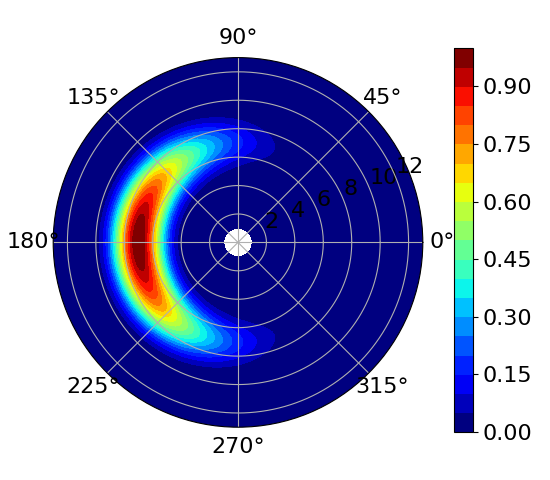
\includegraphics[width=\textwidth]{Figs/initConvergenceConds/Poloidal1}
  \caption{\label{fig::init Poloidal 1}Equation \ref{eq::poloidal init 1}}
 \end{subfigure}
 \hspace{.05\textwidth}
 \begin{subfigure}[t]{.45\textwidth}
  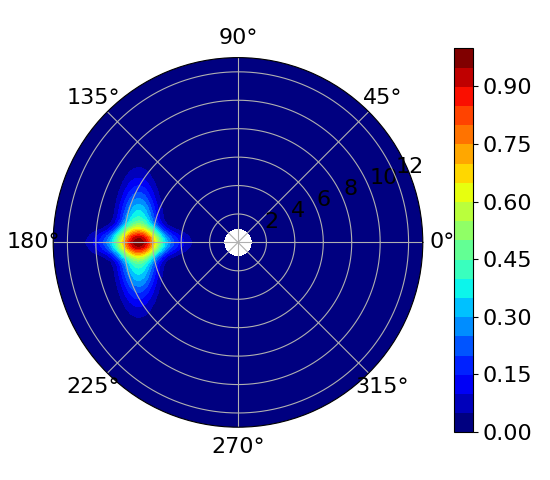
\includegraphics[width=\textwidth]{Figs/initConvergenceConds/Poloidal2}
  \caption{\label{fig::init Poloidal 2}Equation \ref{eq::poloidal init 2}}
 \end{subfigure}
 \caption{\label{fig::init conds poloidal}Initial conditions $f_0$ for the poloidal advection convergence tests as described by equations \ref{eq::poloidal init 1} and \ref{eq::poloidal init 2}}
\end{figure}


Two different initial conditions will be used. The first will be an ellipsis in the coordinates ($r$,$\theta$). The second will not be dependent on the coordinates and will have a more irregular shape as shown in figure \ref{fig::init conds poloidal}. The conditions are defined as follows:
\begin{align}
 f_0(r,\theta)&=B(r_1(r,\theta),a_1) \label{eq::poloidal init 1}\\
 f_0(r,\theta)&=B(r_2(r\cos(\theta),r\sin(\theta),a_2)+B(r_3(r\cos(\theta),r\sin(\theta)),a_2) \label{eq::poloidal init 2}\\
 B(r,a) &= 
 \begin{cases}
  \cos\left(\frac{\pi r}{2 a}\right)^4\quad\quad \text{ if }r\leq a\\
  0\quad\quad\quad \text{otherwise}
 \end{cases}\nonumber\\
r_1(x,y) &= \sqrt{(x-7)^2+2*(y-\pi)^2}\nonumber\\
r_2(x,y) &= \sqrt{(x+7)^2+8*y^2}\nonumber\\
r_3(x,y) &= \sqrt{4*(x+7)^2+0.5*y^2}\nonumber\\
a_1 &= 4\nonumber\\
a_2 &= 6\nonumber
\end{align}
over the domain $\Omega=[0,20]\cross[0,2\pi]$. The boundary conditions are periodic in $\theta$ and such that $f_0(\reel\backslash\Omega)=0$.

\begin{table}[ht]
\centering
 \begin{tabular}{|r c|r c|c|c|c|c|}
  \hline
  \multicolumn{2}{|c|}{\bf N$_x$} & \multicolumn{2}{|c|}{\bf N$_y$} & \bf L$^2$ norm       & \bf Order & \bf L$^\infty$ norm  & \bf Order\\
  \hline
  \hline
  32  & &  32     & & $ 1.79 \cdot 10^{ -3 }$ &       & $ 3.05 \cdot 10^{ -4 }$ &  \\
  \hline
  64  & &  64     & & $ 2.19 \cdot 10^{ -4 }$ &  3.03  & $ 3.71 \cdot 10^{ -5 }$ &  3.04  \\
  \hline
  128  & &  128     & & $ 2.72 \cdot 10^{ -5 }$ &  3.00  & $ 4.61 \cdot 10^{ -6 }$ &  3.01  \\
  \hline
  256  & &  256     & & $ 3.41 \cdot 10^{ -6 }$ &  3.00  & $ 5.75 \cdot 10^{ -7 }$ &  3.00  \\
  \hline
  512  & &  512     & & $ 4.26 \cdot 10^{ -7 }$ &  3.00  & $ 7.19 \cdot 10^{ -8 }$ &  3.00  \\
  \hline
 \end{tabular}
 \caption{\label{Poloidal dx convergence eq1} Spatial convergence for poloidal advection, $N_x\cdot dt = 0.032$ s, $t_{\text{end}}$=0.2s, $f_0$ is given by equation \ref{eq::poloidal init 1}}
\end{table}

\begin{table}[ht]
\centering
 \begin{tabular}{|r c|r c|c|c|c|c|}
  \hline
  \multicolumn{2}{|c|}{\bf N$_x$} & \multicolumn{2}{|c|}{\bf N$_y$} & \bf L$^2$ norm       & \bf Order & \bf L$^\infty$ norm  & \bf Order\\
  \hline
  \hline
  32  & &  32     & & $ 2.01 \cdot 10^{ -1 }$ &       & $ 6.00 \cdot 10^{ -2 }$ &  \\
  \hline
  64  & &  64     & & $ 1.32 \cdot 10^{ -1 }$ &  0.61  & $ 6.34 \cdot 10^{ -2 }$ &  -0.08  \\
  \hline
  128  & &  128     & & $ 1.99 \cdot 10^{ -2 }$ &  2.73  & $ 9.89 \cdot 10^{ -3 }$ &  2.68  \\
  \hline
  256  & &  256     & & $ 2.22 \cdot 10^{ -3 }$ &  3.17  & $ 1.03 \cdot 10^{ -3 }$ &  3.27  \\
  \hline
  512  & &  512     & & $ 2.60 \cdot 10^{ -4 }$ &  3.09  & $ 1.23 \cdot 10^{ -4 }$ &  3.06  \\
  \hline
  1024 & & 1024     & & $ 3.20 \cdot 10^{ -5 }$ &  3.03 & $ 1.51 \cdot 10^{ -5 }$ & 3.02 \\
  \hline
 \end{tabular}
 \caption{\label{Poloidal dx convergence eq2} Spatial convergence for poloidal advection, $N_x\cdot dt = 0.032$ s, $t_{\text{end}}$=0.05s, $f_0$ is given by equation \ref{eq::poloidal init 2}}
\end{table}

To determine the order of convergence the spatial and temporal convergence orders must be treated separately. In order to  determine the spatial convergence the calculated trajectory is used instead of the second order scheme. This means that all errors are due to the interpolation. As a result the convergence order ought to be equal to the order of the spline approximation. Here the function will be approximated by 3rd degree splines.

Tables \ref{Poloidal dx convergence eq1} and \ref{Poloidal dx convergence eq2} confirm this convergence order. Although it should be noted that shapes which are not dependent on the coordinate system require more points in order to achieve a given accuracy and convergence is only seen once the error is sufficiently small.

In order to determine the temporal convergence order a large number of spatial points is used to ensure that the error is dominated by the errors due to the trajectory calculation. The convergence should therefore be second order. This is confirmed by table \ref{Poloidal dt convergence}

\begin{table}[ht]
\centering
 \begin{tabular}{|r c|l|c|c|c|c|}
  \hline
  \multicolumn{2}{|c|}{\bf N$_t$} & \multicolumn{1}{|c|}{\bf dt} & \bf L$^2$ norm       & \bf Order & \bf L$^\infty$ norm  & \bf Order\\
  \hline
  10  & &  0.1     & $ 3.81 \cdot 10^{ -3 }$ &       & $ 9.19 \cdot 10^{ -4 }$ &  \\
  \hline
  20  & &  0.05     & $ 9.43 \cdot 10^{ -4 }$ &  2.01  & $ 2.28 \cdot 10^{ -4 }$ &  2.01  \\
  \hline
  40  & &  0.025     & $ 2.35 \cdot 10^{ -4 }$ &  2.00  & $ 5.71 \cdot 10^{ -5 }$ &  2.00  \\
  \hline
  80  & &  0.0125     & $ 5.88 \cdot 10^{ -5 }$ &  2.00  & $ 1.43 \cdot 10^{ -5 }$ &  2.00  \\
  \hline
  160  & &  0.00625   & $ 1.47 \cdot 10^{ -5 }$ &  2.00  & $ 3.57 \cdot 10^{ -6 }$ &  2.00  \\
  \hline
 \end{tabular}
 \caption{\label{Poloidal dt convergence} Temporal convergence for poloidal advection, with N$_x$ = N$_y$ = 100, endTime = 1s, $f_0$ is given by equation \ref{eq::poloidal init 1}}
\end{table}

\subsection{Flux-surface advection}

The flux-surface advection operator is defined by equation \ref{Eq::Advection1}:

\begin{equation}
 \partial_t f(v_\parallel) + c \grad_\parallel f = 0
\end{equation}

As the trajectory for the flux-surface advection can be calculated exactly, the convergence order ought to depend on a combination of the error due to the spline approximation and the error due to the Lagrange interpolation. A combination of different ordered convergences can be difficult to identify. Therefore for the purpose of the tests a 3-rd degree Lagrange interpolation will be used in place of the 5-th order interpolation. The function will still be approximated by 3rd degree splines. The convergence therefore ought to be of 3-rd order.

The convergence is tested using the following function:
\begin{align}
 f_0(\theta,z)&=B(r_1(r,\theta),a_1) \label{eq::flux init}\\
 B(r,a) &= 
 \begin{cases}
  \cos\left(\frac{\pi r}{2 a}\right)^4\quad\quad \text{ if }r\leq a\\
  0\quad\quad\quad \text{otherwise}
 \end{cases}\nonumber\\
 r_1(x,y) &= \sqrt{(x-10)^2+2*(y-\pi)^2}\nonumber\\
 a_1 &= 4\nonumber
\end{align}
over the domain $\Omega=[0,2\pi]\cross[0,20]$. The boundary conditions are periodic in $\theta$ and such that $f_0(\reel\backslash\Omega)=0$.

This function is chosen as it is $\mathcal{C}^3$ everywhere.

\begin{table}[ht]
\centering
 \begin{tabular}{|r c|r c|l c|c|c|c|c|}
  \hline
  \multicolumn{2}{|c|}{\bf N$_\theta$} & \multicolumn{2}{|c|}{\bf N$_z$} & \multicolumn{2}{|c|}{\bf dt} & \bf L$^2$ norm       & \bf Order & \bf L$^\infty$ norm  & \bf Order\\
  \hline
  32  & &  32  & &  0.1     & & $ 8.26 \cdot 10^{ -2 }$ &       & $ 4.96 \cdot 10^{ -2 }$ &  \\
  \hline
  64  & &  64  & &  0.05     & & $ 1.29 \cdot 10^{ -2 }$ &  2.67  & $ 7.97 \cdot 10^{ -3 }$ &  2.64  \\
  \hline
  128  & &  128  & &  0.025     & & $ 1.70 \cdot 10^{ -3 }$ &  2.93  & $ 1.08 \cdot 10^{ -3 }$ &  2.88  \\
  \hline
  256  & &  256  & &  0.0125     & & $ 2.14 \cdot 10^{ -4 }$ &  2.99  & $ 1.36 \cdot 10^{ -4 }$ &  2.99  \\
  \hline
  512  & &  512  & &  0.00625     & & $ 2.68 \cdot 10^{ -5 }$ &  3.00  & $ 1.71 \cdot 10^{ -5 }$ &  3.00  \\
  \hline
 \end{tabular}
 \caption{\label{Flux dx convergence} Spatial convergence for the flux advection operator with $t_{\text{end}}$ = 1s, $f_0$ as given by equation \ref{eq::flux init}, 3rd degree Lagrange interpolation}
\end{table}

The results can be seen in table \ref{V Parallel convergence}. We see that the convergence is of 3-rd order as expected.

\rchapter{Poisson Equation}

\section{Introduction}

Plasma is quasi-neutral. This means that although locally there may be charged regions, it is neutral overall. This condition is expressed by a Poisson equation. It is therefore important to have a robust and accurate method for solving Poisson equations in order to determine the electric potential.

The independence of the equations in the z-direction will be used to solve multiple equations in parallel. In addition, the method will use Fourier transforms to exploit the periodicity of the solution in the $\theta$-direction in order to obtain further parallelisation.

\section{Quasi-Neutrality Equation}

% \begin{equation}\label{quasi neutrality}
%  -\left[\partial_r^2\phi + \left(\frac{1}{r}+\frac{\partial_rn_0}{n_0}\right)\partial_r\phi+\frac{1}{r^2}\partial_\theta^2\phi\right]+\frac{1}{T_e(r)}\phi=\frac{1}{n_0}\int_{-\infty}^{+\infty}(f-f_{eq})dv_\parallel
% \end{equation}

As discussed in chapter \ref{chapter::Gyrokinetics}, the quasi-neutrality condition can be expressed using the following equation:

\begin{equation}\label{eq::quasi neutrality start}
 -\grad_\perp\cdot\left[\frac{\rho_{m0}}{\varepsilon_0B^2}\grad_\perp\phi\right]+\frac{1}{\lambda_D^2}\left[\phi-\chi\cdot\langle\phi\rangle_f\right]=\frac{1}{\varepsilon_0}\rho_{c1}
\end{equation}

where $\grad_\perp = \left(\grad-\hat{b}\left(\hat{b}\cdot\grad\right)\right)$, $\hat{b}$ is the magnetic unit vector as defined in equation \ref{eq::magnetic unit}, $\rho_{m0}$ is the equilibrium mass density, $\varepsilon_0$ is the permittivity of free space, $B$ is the intensity of the equilibrium background magnetic field, $\phi$ is the electrostatic potential, $\lambda_D$ is the electron Debye length, $\langle\phi\rangle_f$ is the flux-surface average of $\phi$, and $\rho_{c1}$ is the charge perturbation density due to the ions.

As discussed previously, for a torus to be effectively approximated by a straight cylinder, the major radius must be very large. As a result we let $\zeta(r)$ tend to 0. In this limit $\hat{b}$ tends towards $\hat{z}$. This means that the perpendicular gradient can be defined as follows:
\begin{align}
 \grad_\perp\phi=\grad\phi-\hat{b}\left(\hat{b}\cdot\grad\phi\right) \rightarrow& \grad\phi-\hat{z}\left(\hat{z}\cdot\grad\phi\right)\nonumber\\
 =&\partial_r\phi\hat{r}+\frac{1}{r}\partial_\theta\phi\hat{\theta}+\partial_z\phi\hat{z}-\partial_z\phi\hat{z}\nonumber\\
 =& \partial_r\phi\hat{r}+\frac{1}{r}\partial_\theta\phi\hat{\theta}
\end{align}

Defining $g(r)=\frac{\rho_{m0}(r)}{\varepsilon_0B^2}$, the first term in equation \ref{eq::quasi neutrality start} can now be expressed:
\begin{align}
\grad_\perp\left(g\grad_\perp\phi\right)=&\left(\grad-\hat{b}\left(\hat{b}\cdot\grad\right)\right)\cdot\left[g \grad \phi\right]\nonumber\\
\rightarrow& \left(\grad-\hat{z}\left(\hat{z}\cdot\grad\right)\right)\cdot\left[g \partial_r\phi\hat{r}+\frac{g}{r}\partial_\theta\phi\hat{\theta}\right]\nonumber\\
=&\frac{1}{r}\partial_r(rg\partial_r\phi)+\frac{1}{r}\partial_\theta(\frac{g}{r}\partial_\theta\phi)\nonumber\\
=&\frac{g}{r}\partial_r\phi+\partial_r(g\partial_r\phi)+\frac{g}{r^2}\partial_\theta^2\phi\nonumber\\
=&\frac{g}{r}\partial_r\phi+\partial_rg\partial_r\phi+g\partial_r^2\phi+\frac{g}{r^2}\partial_\theta^2\phi)\label{eq::grad perp sq}
\end{align}

Substituting equation \ref{eq::grad perp sq} and the definition of the charge perturbation density due to the ions into equation \ref{eq::quasi neutrality start} and dividing by g then leaves us with the following equation:
\begin{equation}\label{quasi neutrality}
 -\left[\partial_r^2+\left(\frac{1}{r}+\frac{\partial_rg}{g}\right)\partial_r+\frac{1}{r^2}\partial_\theta^2\right]\phi+\frac{1}{g\lambda_D^2}\left[\phi-\chi\cdot\langle\phi\rangle_\theta\right]=\frac{1}{g\varepsilon_0}\rho_{c1}
\end{equation}
where $\rho_{c1}=q_i\int (f-f_{eq})dv$ is the charge perturbation density due to the kinetic species.

This provides a simple differential equation which will be solved using the methods detailed in this chapter.

\section{Fourier Transform}

Fourier transforms decompose functions into the frequencies of which they are composed. This makes them practical for analysing periodic functions. The Fourier transform of a function is defined as followed:

\begin{equation}
 \hat{f}(k)=\mathcal{F}\left[f(x)\right]=\int_{-\infty}^{\infty}f(x)e^{-i k x}dx
\end{equation}

while the inverse Fourier transform is defined as follows:

\begin{equation}
 f(x)=\mathcal{F}^{-1}\left[\hat{f}(k)\right]=\int_{-\infty}^{\infty}\hat{f}(k)e^{i k x}dk
\end{equation}

In addition Fourier transforms have several useful properties. Notably the Fourier transform of a derivative is defined as follows:

$$\widehat{\frac{df}{dx}}(k)=i k \hat{f}(k)$$

The proof of this is shown below:

\begin{align*}
 \widehat{\frac{df}{dx}}(k)&=\mathcal{F}^{-1}\left[\frac{d}{dx}\int_{-\infty}^{\infty}\hat{f}(k)e^{i k x}dx\right]\\
 &=\mathcal{F}^{-1}\left[\int_{-\infty}^{\infty}\hat{f}(k)\frac{d}{dx}e^{i k x}dx\right]\\
 &=\mathcal{F}^{-1}\left[\int_{-\infty}^{\infty}\hat{f}(k)i k e^{i k x}dx\right]\\
 &=i k \hat{f}(k)
\end{align*}

This along with the linearity of the Fourier transform allows equation \ref{quasi neutrality} to be rewritten as follows:

\begin{align*}
 &\mathcal{F}_\theta\left[-\left[\partial_r^2+\left(\frac{1}{r}+\frac{\partial_rg}{g}\right)\partial_r\phi+\frac{1}{r^2}\partial_\theta^2\right]\phi+\frac{1}{g\lambda_D^2}\left[\phi-\chi\cdot\langle\phi\rangle_\theta\right]\right]\\
 =&-\partial_r^2\mathcal{F}_\theta\left[\phi\right] - \left(\frac{1}{r}+\frac{\partial_rg}{g}\right)\partial_r\mathcal{F}_\theta\left[\phi\right]-\frac{1}{r^2}(ik)^2\mathcal{F}_\theta\left[\phi\right]+\frac{1}{g\lambda_D^2}\left[\mathcal{F}_\theta\left[\phi\right]-\chi\delta_{k0}\mathcal{F}_\theta\left[\phi\right]\right]\\
 =&-\partial_r^2\mathcal{F}_\theta\left[\phi\right] - \left(\frac{1}{r}+\frac{\partial_rg}{g}\right)\partial_r\mathcal{F}_\theta\left[\phi\right]+\frac{k^2}{r^2}\mathcal{F}_\theta\left[\phi\right]+\frac{1}{g\lambda_D^2}\left[\mathcal{F}_\theta\left[\phi\right]-\chi\delta_{k0}\mathcal{F}_\theta\left[\phi\right]\right]\\
 =&\frac{1}{g\varepsilon_0}\mathcal{F}_\theta\left[\rho_{c1}\right]
\end{align*}

This leaves us with the following simplified equation which is a one-dimensional differential equation which can be solved using the finite elements method:
\begin{equation}\label{eq::quasi neutrality fourier}
 \left[-\partial_r^2 - \left(\frac{1}{r}+\frac{\partial_rg}{g}\right)\partial_r+\frac{k^2}{r^2}+\frac{1}{g\lambda_D^2}(1-\chi\delta_{k0})\right] \hat{\phi}=\frac{\hat{\rho}}{g\varepsilon_0}
\end{equation}

\section{Finite Elements}\label{sec::FE}

The finite elements method is a numerical method for solving various equations including Poisson equations. It consists of using the representation of functions on a given basis to formulate a matrix equation which can be solved to find the solution to the original equation.

All functions can be represented exactly on an infinite basis however this approach clearly doesn't work in a numerical setting. Instead the solution will be restricted to a subset of functions, with the finite elements method allowing the best approximation in this subset to be found. In this project the basis used will be B-Splines (see section \ref{sec::BSplines}). For a given mode $m$ and a given value of the $z$ coordinate, the solution can therefore be expressed as follows:
\begin{equation}\label{eq::FE discretisation}
\hat{\phi}(r,m,z)=\somme{i=0}{N}c_i\varphi_{i,m,z}(r)
\end{equation}

where $\varphi_{i,m,z}(r)$ is the i-th B-Spline basis for the values of the m and $z$ coordinates, and $c_i$ is the associated coefficient.

The weak form of an equation consists of multiplying it by a test function and integrating over the relevant domain. Any function satisfying the original equation should also satisfy the weak form of the equation for all test functions. If the test functions are chosen such that they form the basis of a function space then the equation stands for any test function in the function space. For this reason the test functions are often chosen to be the basis of the function space on which the solution is approximated.

The weak form of equation \ref{eq::quasi neutrality fourier} is shown below:
\begin{align}
 -\int_\Omega\partial_r^2\hat{\phi}(r,m)\,\psi(r) r\, dr & \nonumber\\
 - \int_\Omega\left(\frac{1}{r}+\frac{\partial_rg(r)}{g(r)}\right) \partial_r\hat{\phi}(r,m)\,\psi(r) r\, dr & \nonumber\\
 + \int_\Omega\left(\frac{k^2}{r^2}+\frac{1}{g(r)\lambda_D(r)^2}(1-\chi\delta_{k0})\right)\hat{\phi}(r,m)\,\psi(r) r\, dr&=\int_\Omega\frac{\hat{\rho}(r,m)}{g\varepsilon_0}\,\psi(r) r\, dr \label{quasi neutrality weak}
\end{align}
where $\Omega$ is the relevant domain, namely $[r_{min},r_{max}]$, $\psi(r)$ is the test function, and $r$ appears in the integral due to the Jacobian of the cylindrical coordinates.

The first term of this equation can be re-expressed as follows:
\begin{align}
 -\int_\Omega\partial_r^2\hat{\phi}(r,m)\,\psi(r)r\, dr =& \left.-\partial_r \hat{\phi}(r,m)\,\psi(r) r \right|_{\partial\Omega}+\int_\Omega\partial_r\hat{\phi}(r,m)\,\partial_r\psi(r)r\, dr\nonumber\\
 &+\int_\Omega\partial_r\hat{\phi}(r,m)\,\psi(r) dr\label{eq::FE boundary}
\end{align}

This avoids the use of high order derivatives which would decrease the accuracy of the solution. It also introduces a boundary term which allows the boundary conditions to be imposed.

In our simulations two types of boundary conditions will be used. These are homogeneous Dirichlet boundary conditions (where the boundary value is fixed at zero) and homogeneous Neumann boundary conditions (where the derivative at the boundary is fixed at zero). In the case of Neumann boundary conditions it is clear that the boundary term is equal to zero. In the case of Dirichlet boundary conditions the boundary term is also zero as long as the function space is restricted to functions which are also equal to zero on the boundary.

Inserting equation \ref{eq::FE boundary} and the basis representation described by equation \ref{eq::FE discretisation} into equation \ref{quasi neutrality weak} gives the following equation:
\begin{align}
 \underset{j}{\sum}\left[\int_\Omega\partial_r\varphi_j(r)\,\partial_r\psi_i(r)r\, dr \right. & \nonumber\\
 +\int_\Omega\partial_r\varphi_j(r)\,\psi_i(r) dr & \nonumber\\
 - \int_\Omega \left(\frac{1}{r}+\frac{\partial_rg(r)}{g(r)}\right)\partial_r\varphi_j(r)\,\psi_i(r)r\, dr & \\
 \left.+ \int_\Omega\left(\frac{k^2}{r^2}+\frac{1}{g(r)\lambda_D(r)^2}(1-\chi\delta_{k0})\right)\varphi_j(r)\,\psi_i(r)r\, dr\right]&c_j=\int_\Omega\frac{\hat{\rho}(r,m)}{g(r)\varepsilon_0}\,\psi_i(r)r\, dr\nonumber
\end{align}

The solution to the problem is therefore the coefficients $c_j$. Everything else can be expressed using the definitions of the B-Splines and a quadrature scheme. The quadrature scheme used in this project is Gauss-Legendre quadrature which is exact for polynomials of degree 2n-1 when n is the number of different points required to calculate the quadrature. This equation can also be expressed in matrix notation, in this case the integral is contained within a matrix $\mat{A}\in\reel^{N\text{x}N}$, known as the stiffness matrix, and defined as follows:
\begin{align}
 \mat{A}_{ij}=&\int_\Omega\partial_r\varphi_j(r)\,\partial_r\psi_i(r)r\, dr +\int_\Omega\partial_r\varphi_j(r)\,\psi_i(r) dr\nonumber\\
 &- \int_\Omega\left(\frac{1}{r}+\frac{\partial_rg(r)}{g(r)}\right) \partial_r\varphi_j(r)\,\psi_i(r)r\, dr\nonumber\\
 &+ \int_\Omega\left(\frac{k^2}{r^2}+\frac{1}{g(r)\lambda_D(r)^2}(1-\chi\delta_{k0})\right)\varphi_j(r)\,\psi_i(r)r\, dr
\end{align}

The right-hand side is a vector $\vec{b}\in\reel^{N}$:
\begin{equation}
 \vec{b}_i = \int_\Omega\frac{\hat{\rho}(r,m)}{g(r)\varepsilon_0}\,\psi_i(r)r\, dr\nonumber
\end{equation}

As mentioned previously $\hat{\rho}$ is the Fourier transform of $\rho_{c1}$ which is defined as follows:
\begin{equation}
 \rho_{c1} = q_i \int (f - f_{eq}) dv
\end{equation}

The values will therefore be calculated at each point for which the value of the distribution function $f$ is stored. These points are the Greville points of a spline function. The result is therefore an approximation of $\hat{\rho}$ in the function space of the splines. As a result it can also be expressed using b-splines:
\begin{equation}\label{eq::rho discretisation}
\hat{\rho}(r,m,z)=\somme{i=0}{N}p_i\varphi_{i,m,z}(r)
\end{equation}

The vector $\vec{b}$ can therefore be rewritten as:
\begin{equation*}
 \vec{b}_i = \underset{j}{\sum}p_j\int_\Omega\frac{1}{g(r)\varepsilon_0} \psi_j(r) \,\psi_i(r)r\, dr
\end{equation*}

The vector can therefore also be expressed in matrix notation. In this case the integral is contained within a matrix $\mat{M}\in\reel^{N\text{x}N}$, known as the mass matrix, and defined as follows:
\begin{equation}
 M_{ij}=\int_\Omega\frac{1}{g(r)\varepsilon_0} \psi_j(r) \,\psi_i(r)r\, dr
\end{equation}


The coefficients $c_j$ are therefore the elements of the vector $\vec{c}\in\reel^N$, solution of the matrix equation $\mat{A}\vec{c}=\mat{M}\vec{p}$

\section{B-Spline}\label{sec::BSplines}

B-splines are a basis of the function space containing splines. A spline $s(x)$ is a piece-wise polynomial function. It is defined by a degree d, and knots $x_0,\dots,x_m$ such that $a_i\leq a_{i+1}$ and $s(x)$ is (d-r) times differentiable at any knot which appears r times\cite{SplineBook}. In this project, the knots for n-th degree splines will always be chosen such that the spline is $\mathcal{C}^{d-1}$. This means that repeated knots can only appear on the boundary of the considered domain.

Every function space can have multiple different bases. B-splines are a specific basis defined as follows:
\begin{gather}
 N_i^0(x)=
 \begin{cases}
  1\quad\quad \text{ if } x\in[x_i,x_{i+1}[\\
  0\quad\quad \text{ otherwise}
 \end{cases}\\
 N_i^{n} = \alpha_i^{n-1}N_i^{n-1}(x)+\left(1-\alpha_{i+1}^{n-1}\right)N_{i+1}^{n-1}(x)\\
 \alpha_i^{n-1}=
 \begin{cases}
  \frac{u-x_i}{x_{i+n}-x_i}\quad\quad \text{ if } x_{i+n}\neq x_i\\
  0\quad\quad\quad \text{ otherwise}
 \end{cases}
\end{gather}

The b-spline basis for 3-rd degree splines can be seen in figure \ref{3rd degree BSplines}. Note that the central splines cover d+1=4 elements $[a_i,a_{i+1}[$. Therefore d+2 knots are required for each basis function. The additional knots required for the functions nearer to the edge of the domain are repeated knots on the boundary; thus $a_0=a_1=\dots=a_d$, and $a_m=a_{m-1}=\dots=a_{m-d}$.

\begin{figure}[ht]
 \centering
 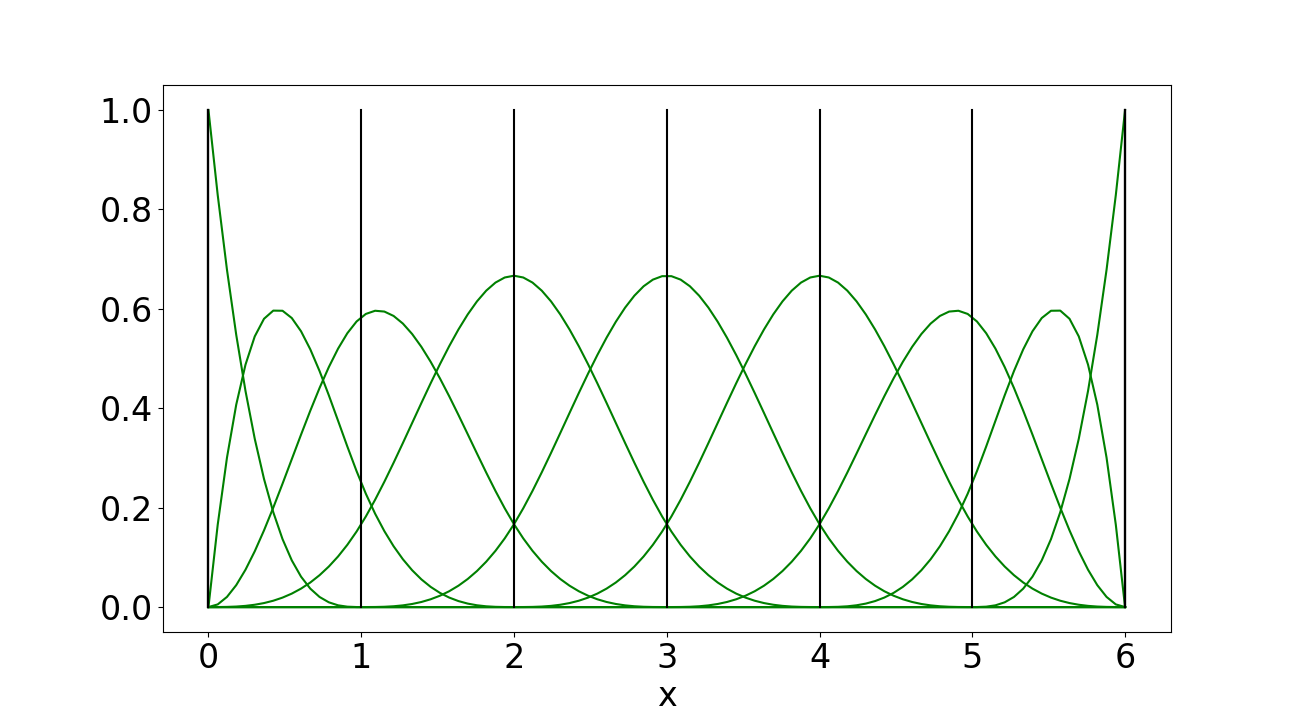
\includegraphics[width=\textwidth]{Figs/bSplines.png}
 \caption{\label{3rd degree BSplines}3rd degree B-Spline with additional knots found on the boundary}
\end{figure}

The d-th degree splines, which make up the function space to which the solution of the Finite Elements problem will belong, can therefore be expressed as follows:
\begin{align}
s(x)=\underset{i}{\sum}c_iN_i^d(x)
\end{align}

The shape of the B-Splines therefore means that the mass and stiffness matrices will be band matrices.

\section{Implementation Details}

The aforementioned schemes will therefore be used to implement equation \ref{quasi neutrality}:
\begin{equation}
 -\left[\partial_r^2+\left(\frac{1}{r}+\frac{\partial_rg}{g}\right)\partial_r+\frac{1}{r^2}\partial_\theta^2\right]\phi+\frac{1}{g\lambda_D^2}\left[\phi-\chi\cdot\langle\phi\rangle_\theta\right]=\frac{1}{g\varepsilon_0}\rho_{c1}
\end{equation}

Note that $g\lambda_D^2=\frac{m\kappa T_e(r)}{B^2q_e^2}$, $\frac{\partial_rg}{g}=\frac{\partial_rn_0}{n_0}$ and $g\varepsilon_0=\frac{mn_0(r)}{B^2}$. For implementation purposes, it is supposed that m=q=1. Thus the following parameters must be provided to complete the problem:
\begin{itemize}
 \item $n_0(r)$
 \item $\partial_rn_0(r)$ (in practice $\frac{\partial_rn_0(r)}{n_0(r)}$ may be provided if it can be expressed more simply)
 \item $B$
 \item $\kappa T_e(r)$
 \item $\chi$
\end{itemize}

In addition an additional parameter will be requested in order to signify whether electrons are considered to be a kinetic or adiabatic species. In the kinetic case it will be assumed that $\frac{1}{\lambda_D^2}=0$.

The above equation is somewhat complicated and it is therefore preferable to implement the following equation:
\begin{equation}
 a\cdot\partial_r^2\phi+b\cdot\partial_r\phi+c\cdot\phi+d\cdot\partial_\theta^2\phi=e\cdot\rho
\end{equation}
where a is a constant and b,c,d and e are any functions dependant on r, in order to be able to test each element of the equation individually. This makes it easier to locate any errors in the scheme.

The following matrices will then be built:
\begin{gather}
 A_{ij}=\int_\Omega a\left(\partial_r\phi_j\partial_r\psi_i r + \partial_r\phi_j\psi_i\right)\, dr\\
 B_{ij}=\int_\Omega b(r)\partial_r\phi_j\psi_i r\, dr\\
 C_{ij}=\int_\Omega c(r)\phi_j\psi_i r\, dr\\
 D_{ij}=\int_\Omega d(r)\phi_j\psi_i r\, dr\\
 E_{ij}=\int_\Omega e(r)\phi_j\psi_i r\, dr
\end{gather}

The solution will therefore be the solution $\vec{\phi}$ to the following matrix equation:
\begin{equation}
 \left(-\mat{A}+\mat{B}+\mat{C}-k^2\mat{D}\right)\vec{\phi}=\mat{E}\vec{\rho}
\end{equation}

As mentioned in section \ref{sec::FE} Dirichlet and Neumann homogeneous boundary conditions will be used. Dirichlet boundary conditions will be imposed by restricting the function space of both the test functions and the solution. Specifically this is done by reducing the basis so that it no longer includes the function which is not zero at the boundary. This means that the solution is no longer expressed as in equation \ref{eq::FE discretisation}, but is instead expressed as follows:
\begin{equation}
\hat{\phi}(r,m,z)=\somme{i=1}{N-1}c_i\varphi_{i,m,z}(r)
\end{equation}

Care should be taken with this formulation as the right hand side is still expressed as in equation \ref{eq::rho discretisation}. This means that the mass matrix is a rectangular matrix.

The boundary conditions used at $r=r_\text{max}$ are always homogeneous Dirichlet conditions. At $r=r_\text{min}$ the boundary conditions are homogeneous Dirichlet conditions for all modes except the 0-th mode where homogeneous Neumann conditions are used.

\section{Convergence}

The convergence order of the scheme described above will be determined by testing the following equation:
\begin{equation}\label{eq::Convergence QN}
 \left[-\partial_{r}^2 - \left[\frac{1}{r} - \kappa_{n_0} \left(1 - \tanh\left( \frac{r - r_p }{\delta_{r_{n_0}}}\right)^2\right)\right]\partial_r + \frac{1}{T_e(r)}-\frac{1}{r^2}\partial_\theta^2\right]\phi = \rho
\end{equation}

The function $\rho$ will be determined by choosing a solution and substituting this into equation \ref{eq::Convergence QN}. The solution chosen will be the following:
\begin{equation}\label{eq::Convergence QN solution}
 \phi(r,\theta)=\cos\left(\frac{3\pi(r-r_{\min})}{2(r_{\max}-r_{\min})}\right)^4\sin(\theta)^3
\end{equation}

The boundary conditions will be Neumann at $r=r_{\min}$ and Dirichlet at $r=r_{\max}$. This solution can be seen in figure \ref{fig::Convergence QN shape}.

Tests have shown that the Fourier transform is exact to machine precision for this function even for small values of $N_\theta$. The results therefore show only the convergence as a function of the number of finite elements in the $r$ direction. We expect that a convergence order of d+1 when splines of degree d are used.

\begin{figure}[b!]
 \centering
 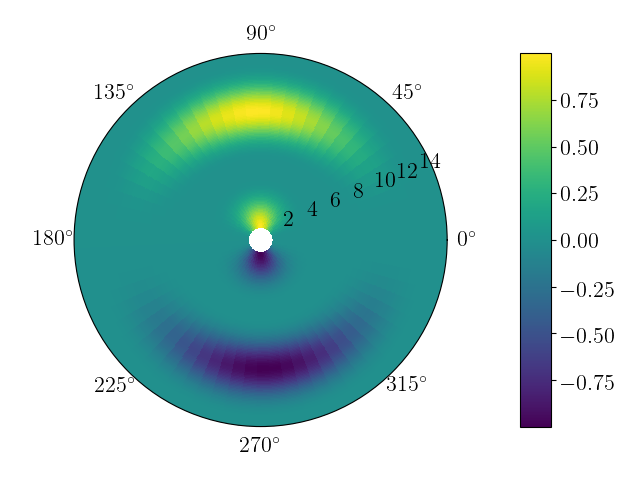
\includegraphics[width=.7\textwidth]{Figs/PoissonConvergence/ExactSolution.png}
 \caption{\label{fig::Convergence QN shape} The form of equation \ref{eq::Convergence QN solution}, the chosen solution of equation \ref{eq::Convergence QN} used to test convergence. $N_r=128$, $N_\theta=64$}
\end{figure}

\begin{table}[p]
 \begin{tabular}{|r c|r c|c|c|c|c|}
 \hline
 \multicolumn{2}{|c|}{\bf Spline} & \multicolumn{2}{|c|}{\bf N$_\text{elem}$} & \bf L$^2$ norm       & \bf Order & \bf L$^\infty$ norm  & \bf Order\\
 \multicolumn{2}{|c|}{\bf degree} &  & &        &  &   & \\
 \hline
 \hline
1  & &  16     & & $ 1.27 \cdot 10^{ -1 }$ &       & $ 4.59 \cdot 10^{ -2 }$ &  \\
\hline
1  & &  32     & & $ 3.28 \cdot 10^{ -2 }$ &  1.95  & $ 1.43 \cdot 10^{ -2 }$ &  1.69  \\
\hline
1  & &  64     & & $ 8.28 \cdot 10^{ -3 }$ &  1.99  & $ 3.91 \cdot 10^{ -3 }$ &  1.87  \\
\hline
1  & &  128     & & $ 2.08 \cdot 10^{ -3 }$ &  2.00  & $ 1.01 \cdot 10^{ -3 }$ &  1.95  \\
\hline
1  & &  256     & & $ 5.19 \cdot 10^{ -4 }$ &  2.00  & $ 2.56 \cdot 10^{ -4 }$ &  1.98  \\
\hline
1  & &  512     & & $ 1.30 \cdot 10^{ -4 }$ &  2.00  & $ 6.44 \cdot 10^{ -5 }$ &  1.99  \\
\hline
1  & &  1024     & & $ 3.25 \cdot 10^{ -5 }$ &  2.00  & $ 1.61 \cdot 10^{ -5 }$ &  2.00  \\
\hline
1  & &  2048     & & $ 8.12 \cdot 10^{ -6 }$ &  2.00  & $ 4.03 \cdot 10^{ -6 }$ &  2.00  \\
\hline
 \hline
2  & &  16     & & $ 9.98 \cdot 10^{ -3 }$ &       & $ 7.40 \cdot 10^{ -3 }$ &  \\
\hline
2  & &  32     & & $ 9.56 \cdot 10^{ -4 }$ &  3.38  & $ 8.11 \cdot 10^{ -4 }$ &  3.19  \\
\hline
2  & &  64     & & $ 9.30 \cdot 10^{ -5 }$ &  3.36  & $ 6.92 \cdot 10^{ -5 }$ &  3.55  \\
\hline
2  & &  128     & & $ 9.41 \cdot 10^{ -6 }$ &  3.30  & $ 5.75 \cdot 10^{ -6 }$ &  3.59  \\
\hline
2  & &  256     & & $ 1.05 \cdot 10^{ -6 }$ &  3.16  & $ 5.45 \cdot 10^{ -7 }$ &  3.40  \\
\hline
2  & &  512     & & $ 1.26 \cdot 10^{ -7 }$ &  3.06  & $ 6.02 \cdot 10^{ -8 }$ &  3.18  \\
\hline
2  & &  1024     & & $ 1.56 \cdot 10^{ -8 }$ &  3.02  & $ 7.09 \cdot 10^{ -9 }$ &  3.09  \\
\hline
2  & &  2048     & & $ 1.94 \cdot 10^{ -9 }$ &  3.00  & $ 8.60 \cdot 10^{ -10 }$ &  3.04  \\
\hline
 \hline
3  & &  16     & & $ 2.38 \cdot 10^{ -3 }$ &       & $ 8.76 \cdot 10^{ -4 }$ &  \\
\hline
3  & &  32     & & $ 2.00 \cdot 10^{ -4 }$ &  3.57  & $ 1.51 \cdot 10^{ -4 }$ &  2.54  \\
\hline
3  & &  64     & & $ 2.50 \cdot 10^{ -5 }$ &  3.00  & $ 2.21 \cdot 10^{ -5 }$ &  2.77  \\
\hline
3  & &  128     & & $ 2.30 \cdot 10^{ -6 }$ &  3.45  & $ 2.20 \cdot 10^{ -6 }$ &  3.33  \\
\hline
3  & &  256     & & $ 1.74 \cdot 10^{ -7 }$ &  3.73  & $ 1.75 \cdot 10^{ -7 }$ &  3.65  \\
\hline
3  & &  512     & & $ 1.19 \cdot 10^{ -8 }$ &  3.87  & $ 1.24 \cdot 10^{ -8 }$ &  3.82  \\
\hline
3  & &  1024     & & $ 7.78 \cdot 10^{ -10 }$ &  3.93  & $ 8.23 \cdot 10^{ -10 }$ &  3.91  \\
\hline
3  & &  2048     & & $ 4.99 \cdot 10^{ -11 }$ &  3.96  & $ 5.32 \cdot 10^{ -11 }$ &  3.95  \\
\hline
 \hline
4  & &  16     & & $ 4.41 \cdot 10^{ -4 }$ &       & $ 1.76 \cdot 10^{ -4 }$ &  \\
\hline
4  & &  32     & & $ 1.88 \cdot 10^{ -5 }$ &  4.55  & $ 1.61 \cdot 10^{ -5 }$ &  3.45  \\
\hline
4  & &  64     & & $ 1.04 \cdot 10^{ -6 }$ &  4.18  & $ 9.28 \cdot 10^{ -7 }$ &  4.12  \\
\hline
4  & &  128     & & $ 3.45 \cdot 10^{ -8 }$ &  4.91  & $ 3.19 \cdot 10^{ -8 }$ &  4.86  \\
\hline
4  & &  256     & & $ 8.17 \cdot 10^{ -10 }$ &  5.40  & $ 7.63 \cdot 10^{ -10 }$ &  5.38  \\
\hline
4  & &  512     & & $ 1.62 \cdot 10^{ -11 }$ &  5.66  & $ 1.53 \cdot 10^{ -11 }$ &  5.64  \\
\hline
4  & &  1024     & & $ 3.00 \cdot 10^{ -13 }$ &  5.75  & $ 2.79 \cdot 10^{ -13 }$ &  5.78  \\
\hline
 \end{tabular}
\caption{\label{tab::Convergence QN} Convergence of the Finite Elements method for equation \ref{eq::Convergence QN} with $N_\theta=8$}
\end{table}

The results are shown in table \ref{tab::Convergence QN}, and figure \ref{fig::Convergence QN}. It can be seen that the 1st degree spline approximation converges with the expected order, while the 2nd and 3rd degree spline approximations converge to the correct order. The 4th degree spline approximation has approximately the correct order however it is hard to gain conclusive evidence as the error quickly approaches machine precision which causes errors which are not due to the method.

\begin{figure}[h]
 \centering
 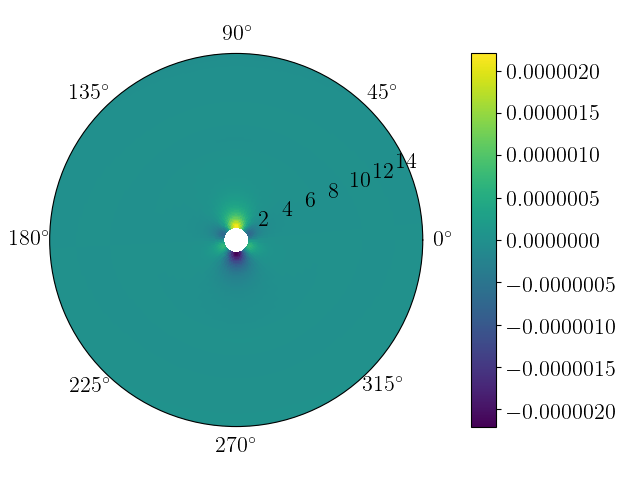
\includegraphics[width=.65\textwidth]{Figs/PoissonConvergence/Error.png}
 \caption{\label{fig::Convergence QN Error} Error of the solution of equation \ref{eq::Convergence QN}, where the exact solution is specified by equation \ref{eq::Convergence QN solution}. Note that most errors are found near the Neumann boundary.}
\end{figure}

\begin{figure}[h]
 \centering
 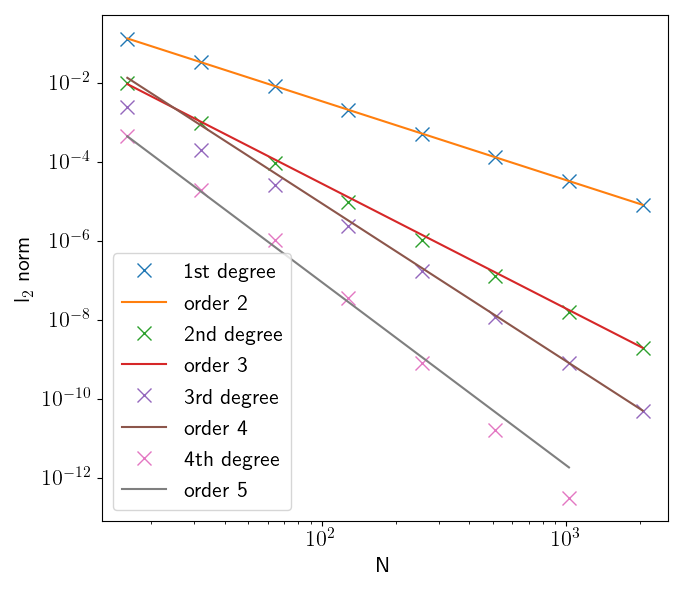
\includegraphics[width=.69\textwidth]{Figs/PoissonConvergence/l2_elementwise.png}
 \vspace{-1em}
 \caption{\label{fig::Convergence QN} Convergence of the Finite Elements method for equation \ref{eq::Convergence QN}. Exact values can be found in table \ref{tab::Convergence QN}}
\end{figure}


\rchapter{Parallel Setup}

\section{Introduction}

Gyrokinetic equations are defined in at least four dimensions. This means that even if a small number of points is used in each dimension, the resulting grid will have a very large number of points. In addition the non-linear nature of the equation means that for most dimensions, an accurate solution cannot be obtained from a very small number of points. Operations on such a high volume of data can be very time consuming. It is therefore important to ensure that parallelisation is used wherever possible.

Parallelisation allows independent calculations to be carried out simultaneously. This decreases the time required to calculate the final solution as the solution at multiple points in the data can be calculated simultaneously. For this method to be effective, it is important that as much of the calculation as possible can be carried out independently. If data stored on a different process is required to complete the calculation then the exchange of data will dramatically increase the overhead, slowing down the calculation time. This can negate the improvement achieved by parallelisation and should therefore be avoided wherever possible. This means that if a calculation requires values from multiple points along one dimension, then ideally that dimension should not be distributed.

This highlights a second consideration: the organisation of the data in memory. Different configurations of the data can lead to different memory latency. If data is accessed contiguously then the loading of cache lines and prefetching (which can be carried out easily by the system as the access pattern is easily recognisable) will ensure that the subsequently required data is already found on a cache. This is important as cache misses can be very costly. The further the data must travel before it can be used, the greater the latency. Optimal memory access is especially important as calculations are often memory-bound rather than compute-bound due to the increase in CPU power following Moore's law and the lack of improvement in memory latency.

It is therefore important to manage access to data structures in an efficient way to ensure that calculations can be carried out as quickly and easily as possible. This should be carried out using parallelisation as well as an optimal arrangement of the data in memory.

In this chapter effective ways of managing the data to fulfil these criteria will be examined.

\section{Choosing layouts}

The arrangement of the data in memory depends on the requirements of the calculations. The screw-pinch model with cylindrical geometry is characterised by 3 operators which arise from the following three advection equations:

\begin{align}
 \partial_t f + v_\parallel \nabla_\parallel f &= 0 \label{eq::Advection1}\\
 \partial_t f + \nabla_\parallel \tilde{\phi} \partial_{v_{\parallel}} f &= 0 \label{eq::Advection2}\\
 \partial_t f + \{\tilde{\phi}, f\} &= 0 \label{eq::Advection3}
\end{align}

Equation \ref{eq::Advection1} leads to an operator which acts on the particle distribution function f, along the flux surface. This surface is defined on $\eta_2$ and $\eta_3$ so the memory access for these variables ought to be contiguous for this operator. Equation \ref{eq::Advection2} leads to an operator which acts on the distribution function along the velocity or $\eta_4$. Therefore  the memory access for $\eta_4$ ought to be contiguous for this operator. Equation \ref{eq::Advection3} leads to an operator which acts on the distribution function along the poloidal surface. This surface is defined on $\eta_1$ and $\eta_2$ so the memory access for these variables ought to be contiguous for this operator.

Evidently it is not possible to find a structure which is optimal for all three of these operators, however given the amount of calculation involved with each step it is reasonable to change layout between each operator. This has been done previously by Latu et al, 2007 \cite{Gysela5D}. A setup must therefore be found such that the following requirements are met:

\begin{tcolorbox} [enhanced,title=Requirements,attach boxed title to top left={xshift=10pt,yshift=-\tcboxedtitleheight/2},boxed title style={size=small}]

\begin{enumerate}
 \item The number of processes that can be used is maximised \label{Condition Max nprocs}
 \item The dimensions used by the operator are not distributed  \label{Condition distribution}
 \item The dimensions used by the operator are contiguous \label{Condition contiguous}
 \item The number of MPI messages sent and received is minimised \label{Condition MPI overhead}
 \item The memory required is minimised \label{Condition memory}
 \item After setup no memory is allocated \label{Condition allocation}
 \item As little copying of data as possible is used \label{Condition copying}
\end{enumerate}

\end{tcolorbox}

With no other requirements, the maximum number of processes possible is equal to the number of grid points. However requirement \ref{Condition distribution} inhibits requirement \ref{Condition Max nprocs}. Thus the maximum number of processes possible for a given layout is the product of the number of points in each dimension not being used by the operator. In order to achieve a good load balance, the number of processes used in each operation should be the same. Thus the maximum number of processes that can be used at any one time is:

$$max\_procs = \min\{n_{\eta_1}\!\!\cdot n_{\eta_4},\, \, \, n_{\eta_1}\!\!\cdot n_{\eta_2}\!\! \cdot n_{\eta_3},\, \, \, n_{\eta_3}\!\!\cdot n_{\eta_4}\}$$

\begin{table}
\centering
 \begin{tabular}{|c|c|}
  \hline
  Dimension & Number of points\\
  \hline
  $\eta_1$ & 256\\
  \hline
  $\eta_2$ & 512\\
  \hline
  $\eta_3$ & 32\\
  \hline
  $\eta_4$ & 128\\
  \hline
 \end{tabular}
 \caption{\label{tab::Grid example} Example configuration of data points}
\end{table}

Using the example setup in table \ref{tab::Grid example}, it can be seen that in this situation the maximum number of processes would be $n_{\eta_3}\!\!\cdot n_{\eta_4} = 4096$. This shows that it does not make sense to distribute this example in more than two dimensions. Even if we tried to take advantage of being able to distribute in three dimensions for equation \ref{eq::Advection2}, it would be unlikely that this would significantly increase the total number of processes that could be used, as in general $n_{\eta_4}\ll n_{\eta_1}\cdot n_{\eta_2}$. In addition it is often the case that $n_{\eta_4}< n_{\eta_1}$ and $n_{\eta_4}<\cdot n_{\eta_2}$ which would mean that no gains in the total number of processes would be made. Thus the increase in complexity does not justify the possible gains. 

The example setup in table \ref{tab::Grid example} also shows that it makes sense to aim for a distribution in two dimensions. The maximum number of processes that can be used in this case ($n_{\eta_3}\!\!\cdot n_{\eta_4} = 4096$) is significantly larger than the maximum number of processes that could be used if the data was only distributed in one dimension ($\eta_4=128$). Therefore the two dimensional distribution is optimal, unless it causes very large overhead thus violating requirement \ref{Condition MPI overhead}.

This therefore leaves us with the possible configurations shown in table \ref{tab::Possible Ordering}. This ordering is such that non-distributed dimensions are always in the final indices, thus satisfying requirement \ref{Condition contiguous}.

\begin{table}[ht]
\centering
 \begin{tabular}{|c|c|}
  \hline
  Accessing scheme & Possible Ordering\\
  \hline
  Flux surface & $(\eta_1,\eta_4,\eta_2,\eta_3)$\\
               & $(\eta_4,\eta_1,\eta_2,\eta_3)$\\
               & $(\eta_1,\eta_4,\eta_3,\eta_2)$\\
               & $(\eta_4,\eta_1,\eta_3,\eta_2)$\\
  \hline
  V-parallel surface & $(\eta_1,\eta_2,\eta_3,\eta_4)$\\
                     & $(\eta_1,\eta_3,\eta_2,\eta_4)$\\
                     & $(\eta_2,\eta_1,\eta_3,\eta_4)$\\
                     & $(\eta_2,\eta_3,\eta_1,\eta_4)$\\
                     & $(\eta_3,\eta_1,\eta_2,\eta_4)$\\
                     & $(\eta_3,\eta_2,\eta_1,\eta_4)$\\
  \hline
  Poloidal surface & $(\eta_3,\eta_4,\eta_1,\eta_2)$\\
                   & $(\eta_4,\eta_3,\eta_1,\eta_2)$\\
                   & $(\eta_3,\eta_4,\eta_2,\eta_1)$\\
                   & $(\eta_4,\eta_3,\eta_2,\eta_1)$\\
  \hline
 \end{tabular}
 \caption{\label{tab::Possible Ordering} Plausible orderings of dimensions in the three different layouts}
\end{table}

In order to simplify the problem, additional restrictions are placed on the setup. Firstly it is assumed that $\eta_2$ is never distributed, as in any case there is only one setup in which it could be distributed. This has no effect on the preceding discussion. In addition it is assumed that $\eta_2$ will always be in the same position in the ordering. As $\eta_4$ must be contiguous for the operator associated with equation \ref{eq::Advection2}, $\eta_2$ must therefore always be in the third position. This leaves two possible orderings. The choice between the two is arbitrary (the only difference is that the ordering in the first and second positions are exchanged). The choice made here can be seen in table \ref{tab::Ordering}.

\begin{table}[ht]
\centering
 \begin{tabular}{|c|c|}
  \hline
  Accessing scheme & Ordering\\
  \hline
  Flux surface & $(\eta_1,\eta_4,\eta_2,\eta_3)$\\
  \hline
  V-parallel surface & $(\eta_1,\eta_3,\eta_2,\eta_4)$\\
  \hline
  Poloidal surface & $(\eta_4,\eta_3,\eta_2,\eta_1)$\\
  \hline
 \end{tabular}
 \caption{\label{tab::Ordering} The chosen ordering for the three different layouts}
\end{table}

Using this ordering, it is important to find a method for changing layouts which respects requirements \ref{Condition memory}, \ref{Condition allocation}, \ref{Condition copying}, and especially \ref{Condition MPI overhead}.

\section{Moving between layouts}

It is clear from the ordering in table \ref{tab::Ordering} that at each change of layout: $\eta_2$ is untouched, one dimension must become distributed, one dimension must become contiguous and one dimension must not be touched unless the number of processes along that axis changes. The problem can therefore be simplified further by assuming that this will not happen. In other words, in a given distribution direction, at any given moment, the data will be distributed over the same number of processes in that direction. The only difference will be which dimension is stored along that axis in memory (ie. for the ordering in table \ref{tab::Ordering}, $\eta_1$ or $\eta_4$ on the first storage axis will each be distributed over the same number of processes).
%In other words, the number of processes available along each axis will remain constant throughout the simulation, and only which variable is represented by that axis will vary.
As $\eta_2$ does not vary the problem can therefore be visualised in three dimensions as shown in figure \ref{fig::Cartesian}. It should be noted that these decisions have removed some flexibility from our system. In particular, it should be noted that it is impossible to move from a poloidal surface to a flux surface without either first changing to a $v_\parallel$ surface or changing the ordering of the variables in the flux surface.


\begin{figure}[ht]
 \begin{center}
 \begin{subfigure}[t]{.45\textwidth}
  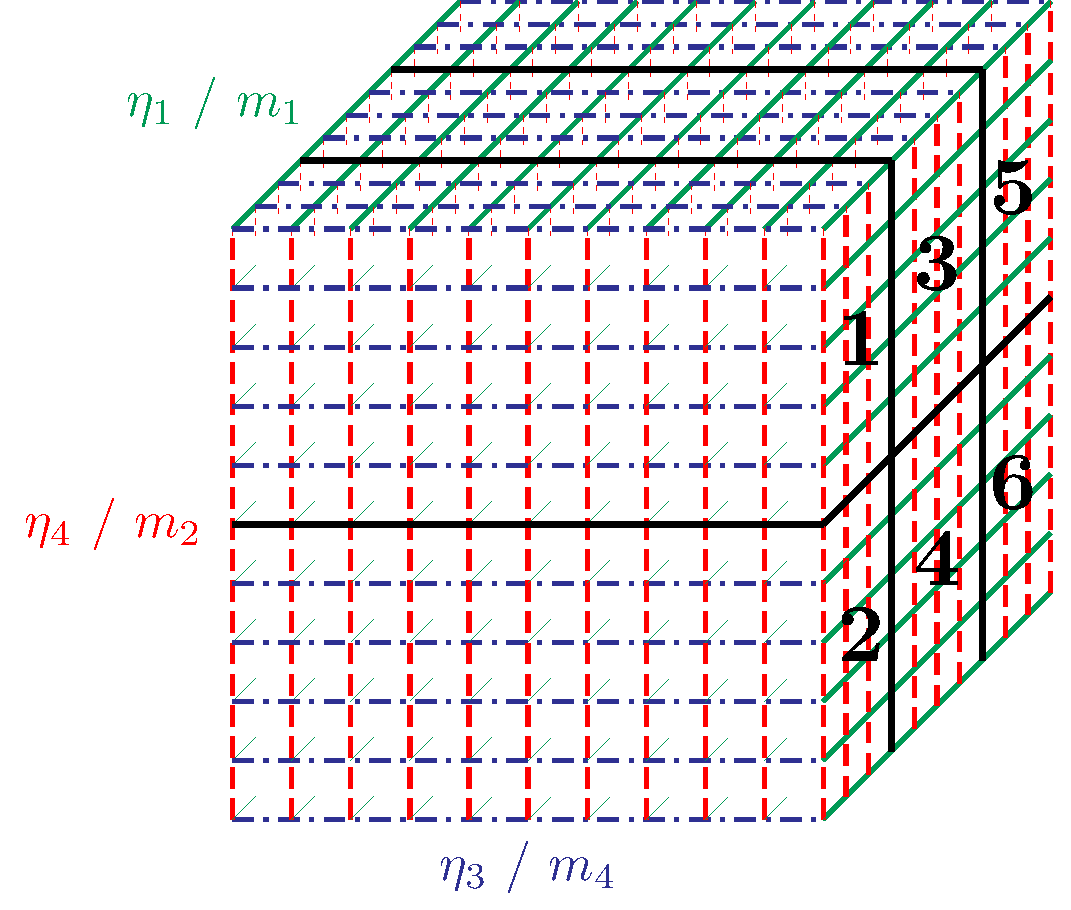
\includegraphics[width=\textwidth]{Figs/ParallelDivision/FluxSurface}
  \caption{\label{fig::FluxSurface}Flux surface - contiguous in z}
 \end{subfigure}
 \hspace{.05\textwidth}
 \begin{subfigure}[t]{.45\textwidth}
  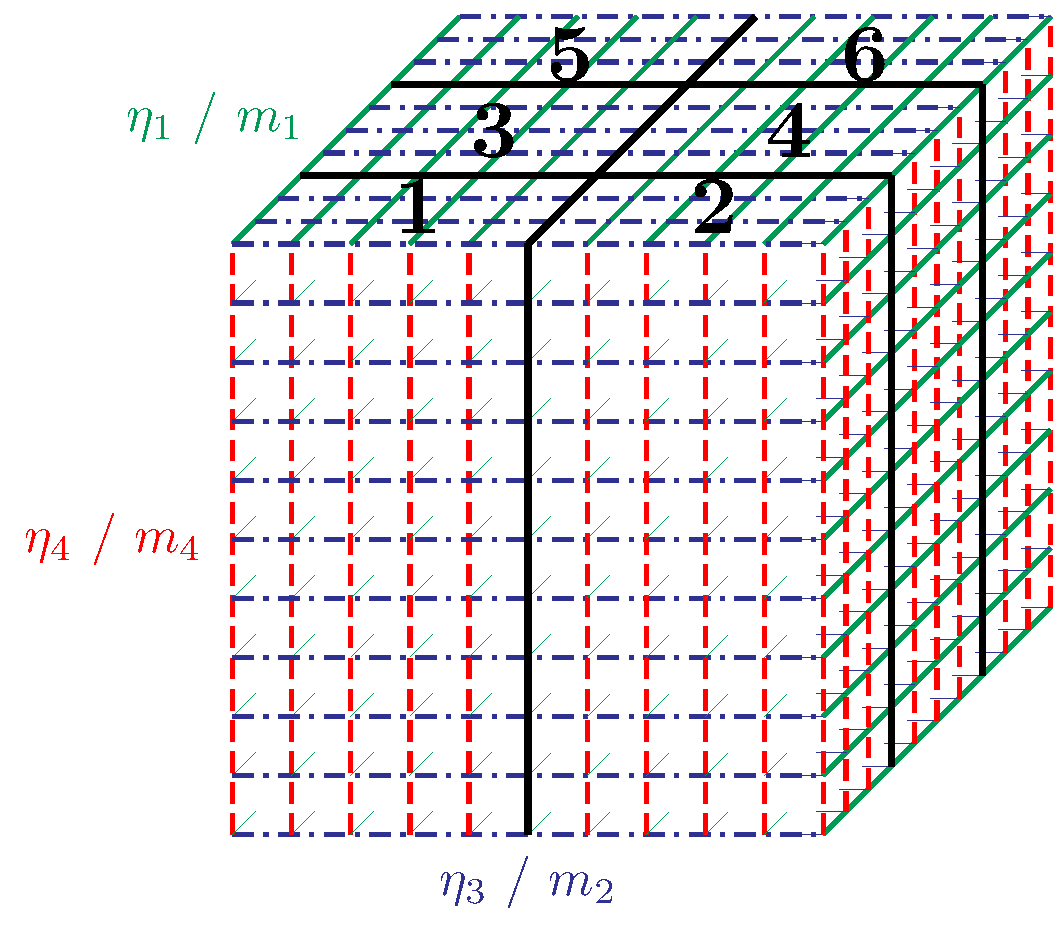
\includegraphics[width=\textwidth]{Figs/ParallelDivision/VParSurface}
  \caption{\label{fig::VPar}$v_\parallel$ surface - contiguous in $v_\parallel$}
 \end{subfigure}
 \begin{subfigure}[t]{.45\textwidth}
  \vspace{1em}
  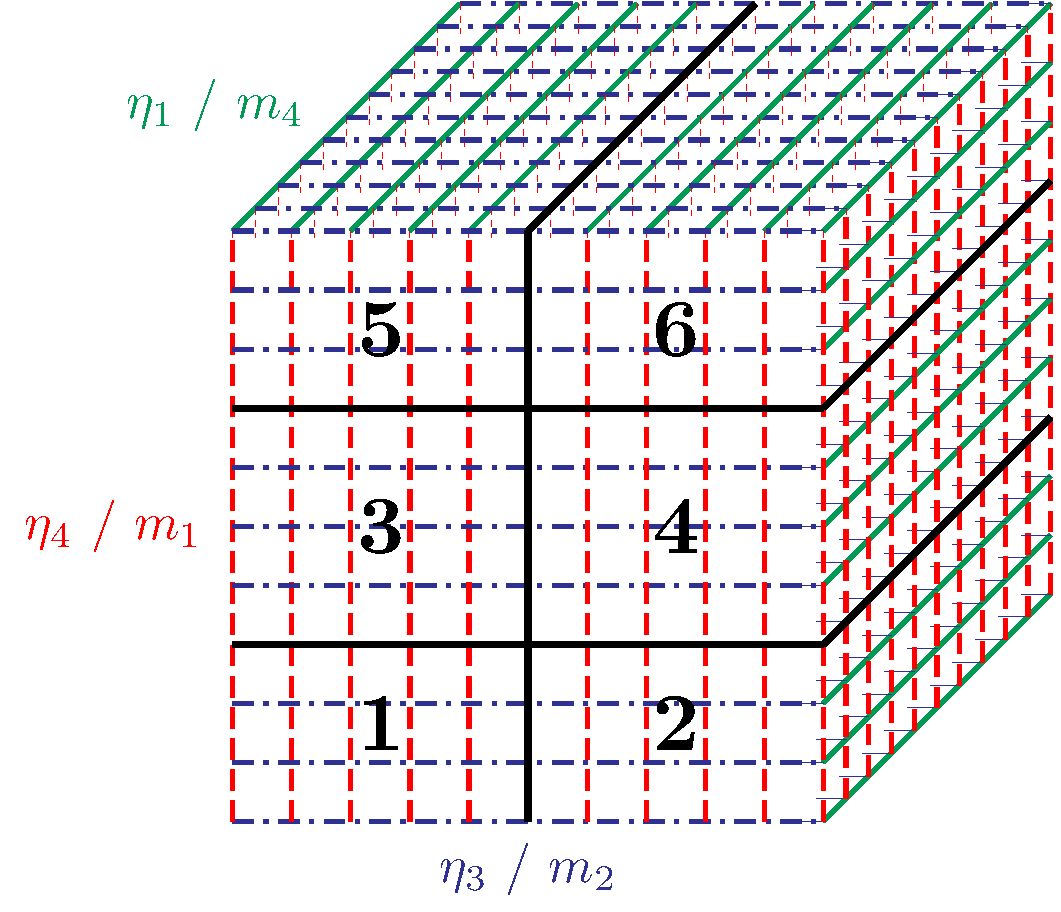
\includegraphics[width=\textwidth]{Figs/ParallelDivision/PoloidalSurface}
  \caption{\label{fig::Poloidal}Poloidal surface - contiguous in r}
 \end{subfigure}
  \caption{\label{fig::Cartesian} 3-D visualisation of the layout change problem. The axis along which the data is stored in memory is indicated by $m_1,m_2,m_4$ ($m_3$ is not represented as it always contains all values of $\eta_2$). Note that the storage axis only changes when the distribution pattern along that axis changes.}
 \end{center}
\end{figure}

Figure \ref{fig::Cartesian} shows three different layouts and allows the viewer to visualise the movement of data between processes during a layout change. Consider the change from the flux-surface layout (figure \ref{fig::FluxSurface}) to the $v_\parallel$ surface layout (figure \ref{fig::VPar}). Process 1 and process 2 must exchange data with one another, however no data is required from any of the other processes. This is also the case for processes 3 and 4, and processes 5 and 6. Similarly when changing from the $v_\parallel$ surface layout to the poloidal surface layout (\ref{fig::Poloidal}) processes 1, 3, and 5 must exchange data only with one another. Indeed, with the conditions imposed each three dimensional layout change is equivalent to multiple independent two dimensional layout changes.

This property can be exploited using an MPI Cartesian grid. This allows the number of messages sent to be greatly reduced thus fulfilling requirement \ref{Condition MPI overhead}. If all processes exchange data amongst themselves, then $p^2$ messages are exchanged,  where $p$ is the total number of processes. In the setup described here, for a grid distributed along a $n \times m$ grid of processes ($nm=p$), changing the variable represented by the first storage axis requires $m n^2$ messages, and changing the variable represented by the second storage axis requires $n m^2$ messages.

In addition the reduced problem can be expressed in one MPI collective command on a sub-communicator: Alltoall. This allows us to use the algorithms provided by MPI rather than relying on multiple point to point messages. This will almost always result in a better optimisation of the code as the MPI implementation can be optimised for hardware.

\subsection{Practical Implementation}

The different layouts each have different memory requirements. This would appear to mean that in order to fulfil requirement \ref{Condition allocation} (after setup no memory is allocated), one array must be allocated for each layout. However this is not ideal as indicated by requirement \ref{Condition memory}. In order to improve this situation, views on numpy arrays are used to access the data. Numpy arrays consists of a 1D array storage and a set of values representing the step-size between consecutive elements in the same dimension. A numpy view is a numpy array where the data has been stored by a different array. Using views therefore allows the allocation of a single one-dimensional array containing the maximum amount of memory required by any given layout. The view then points to a subset of this memory and allows it to be accessed as a multi-dimensional array.

\begin{figure}[ht]
 \begin{center}
 \begin{subfigure}[t]{0.4\textwidth}
  \centering
  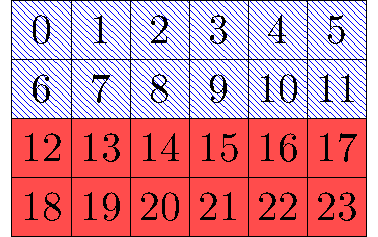
\includegraphics[width=\textwidth]{Figs/SplitConcat2D/Layout1}
  \caption{\label{fig::SplitConcat layout1}Layout 1}
 \end{subfigure}
 \hspace{0.05\textwidth}
 \begin{subfigure}[t]{0.5\textwidth}
  \centering
  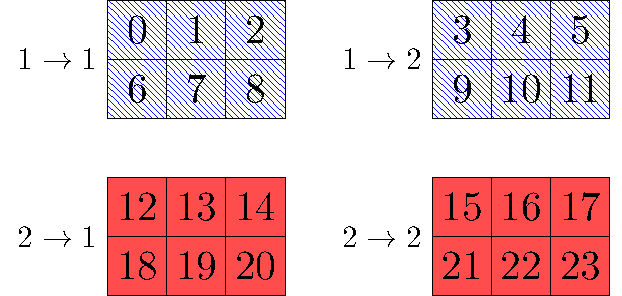
\includegraphics[width=\textwidth]{Figs/SplitConcat2D/SendBlocks}
  \caption{\label{fig::SplitConcat send blocks}Blocks to be sent. These must be copied to a buffer in order to be contiguous by block in memory}
 \end{subfigure}
 \begin{subfigure}[t]{0.5\textwidth}
  \centering
  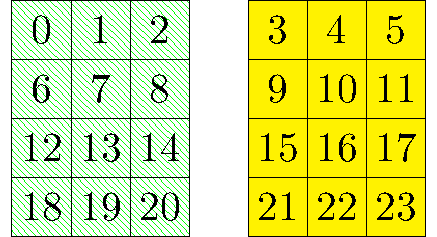
\includegraphics[width=\textwidth]{Figs/SplitConcat2D/RecvLayout}
  \caption{\label{fig::SplitConcat recv blocks}Blocks that are received. These are contiguous but the dimensions are not correctly ordered}
 \end{subfigure}
 \hspace{0.05\textwidth}
 \begin{subfigure}[t]{0.4\textwidth}
  \centering
  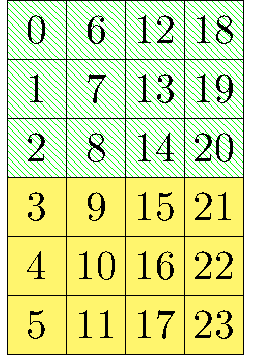
\includegraphics[width=.5\textwidth]{Figs/SplitConcat2D/Layout2}
  \caption{\label{fig::SplitConcat layout2} Layout 2}
 \end{subfigure}
 \begin{subfigure}[t]{\textwidth}
  \centering
  \vspace{1em}
  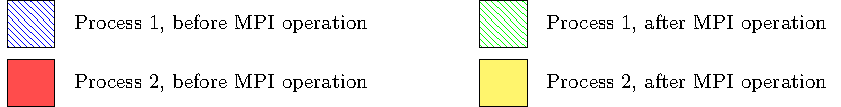
\includegraphics[width=.9\textwidth]{Figs/SplitConcat2D/Legend}
 \end{subfigure}
  \caption{\label{fig::SplitConcat} 2-D visualisation of the layout change algorithm.}
 \end{center}
\end{figure}

When the layout is changed a second array is required for the data to be received. With careful management no additional memory should be required, thus fulfilling requirement \ref{Condition memory}.

Note that the numpy views used for each layout will be different as the dimensions represented by each storage axis change. This can be seen in figure \ref{fig::Cartesian}, but is shown more clearly in figure \ref{fig::Division in memory}.

\begin{figure}[ht]
 \centering
 \begin{subfigure}[t]{0.45\textwidth}
  \centering
  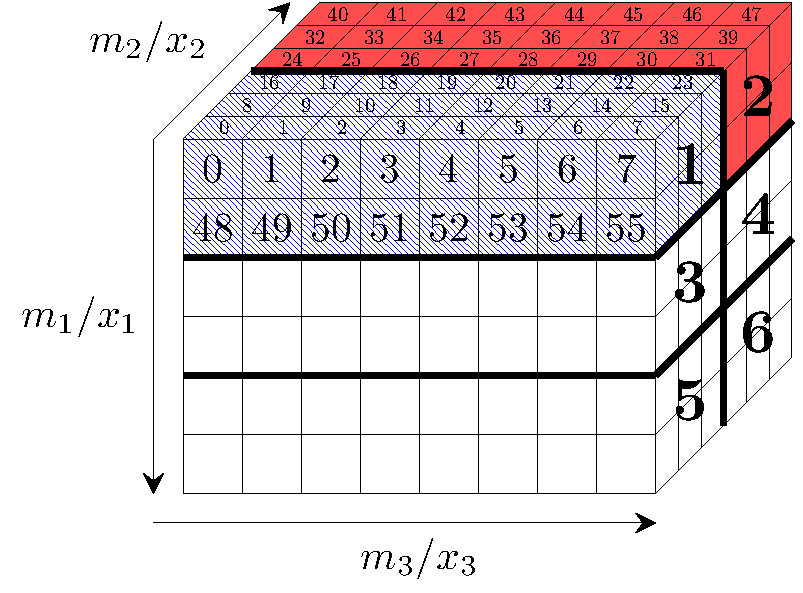
\includegraphics[width=\textwidth]{Figs/DivisionInMemory/FluxSurface}
  \caption{\label{fig::Division in memory Flux} Layout 1}
 \end{subfigure}
 \hspace{0.05\textwidth}
 \begin{subfigure}[t]{0.4\textwidth}
  \centering
  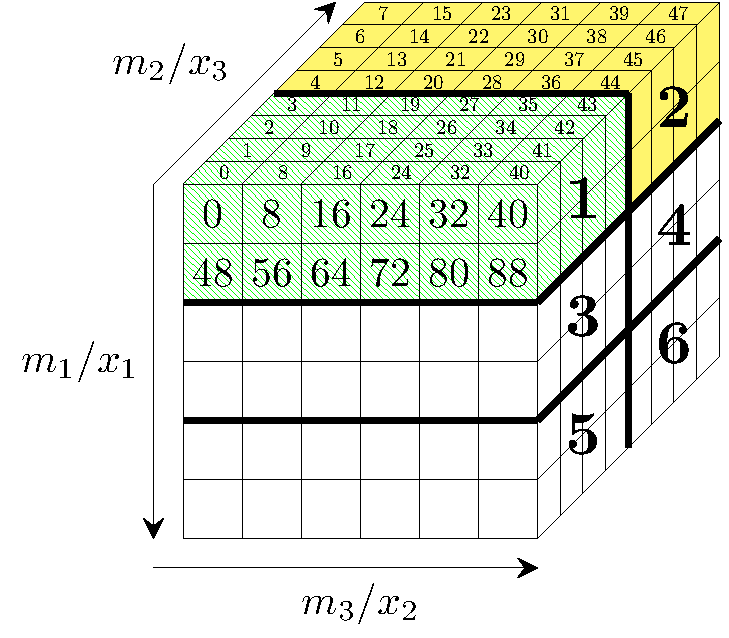
\includegraphics[width=\textwidth]{Figs/DivisionInMemory/VPar}
  \caption{\label{fig::Division in memory VPar} Layout 2}
 \end{subfigure}
 \caption{\label{fig::Division in memory}Different layout arrangements in memory. Note that when the layout changes the shape of the data in memory changes (Colouring is relevant for figure \ref{fig::3D layout change})}
\end{figure}

\begin{figure}[p]
 \begin{center}
 \begin{subfigure}[t]{0.45\textwidth}
  \centering
  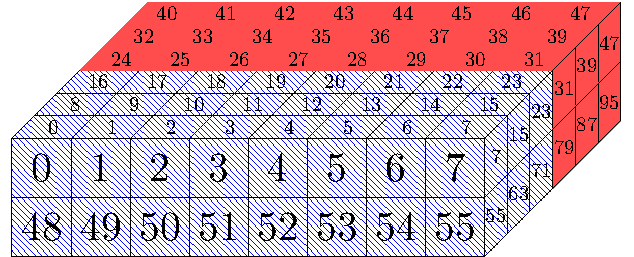
\includegraphics[width=\textwidth]{Figs/SplitConcat3D/Layout1}
  \caption{Layout 1}
 \end{subfigure}
 \hspace{0.05\textwidth}
 \begin{subfigure}[t]{0.45\textwidth}
  \centering
  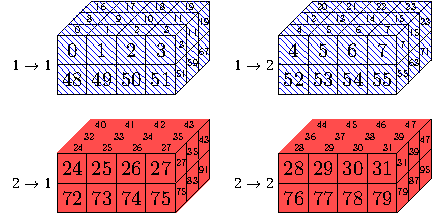
\includegraphics[width=\textwidth]{Figs/SplitConcat3D/SendBlocks}
  \caption{\label{fig::3DSplitConcat send blocks} Blocks to be sent. These must be copied to a buffer in order to be contiguous by block in memory}
 \end{subfigure}
 
 \begin{subfigure}[t]{0.45\textwidth}
  \centering
  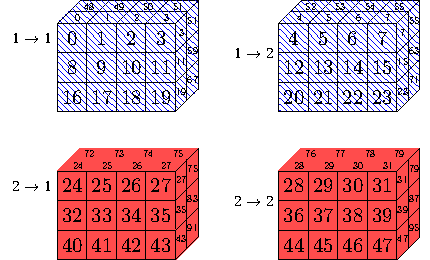
\includegraphics[width=\textwidth]{Figs/SplitConcat3D/TransposedSendBlocks}
  \caption{\label{fig::3DSplitConcat send blocks T}Before sending, the blocks are rearranged so that the axis which was previously distributed becomes the axis with the largest step size (the first axis)}
 \end{subfigure}
 \hspace{0.05\textwidth}
 \begin{subfigure}[t]{0.45\textwidth}
  \centering
  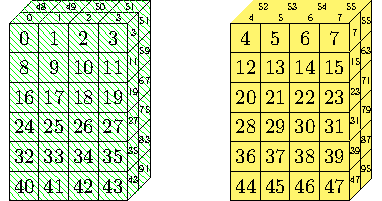
\includegraphics[width=\textwidth]{Figs/SplitConcat3D/RecvLayout}
  \caption{\label{fig::3DSplitConcat recv blocks}Blocks that are received. These are contiguous but the dimensions are not correctly ordered}
 \end{subfigure}
 
 \begin{subfigure}[t]{0.45\textwidth}
  \centering
  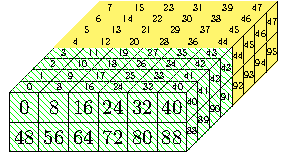
\includegraphics[width=\textwidth]{Figs/SplitConcat3D/Layout2}
  \caption{\label{fig::3DSplitConcat layout2} Layout 2}
 \end{subfigure}
 \hspace{0.05\textwidth}
 \begin{subfigure}[t]{0.45\textwidth}
  \centering
  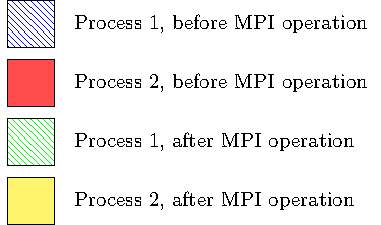
\includegraphics[width=.9\textwidth]{Figs/SplitConcat3D/Legend}
 \end{subfigure}
  \caption{\label{fig::3D layout change} 3-D visualisation of the layout change algorithm. The figure shows the steps for moving the data on processes 1 and 2 from the layout described in figure \ref{fig::Division in memory Flux} to the layout described in figure \ref{fig::Division in memory VPar}}
 \end{center}
\end{figure}

The remaining requirement is requirement \ref{Condition copying} regarding the copying of data. In an ideal implementation the data involved would only be copied once, when it is sent. However unfortunately this is not possible with the layouts described above. The reason for this is illustrated in figure \ref{fig::SplitConcat}. The data is stored in such a way that it is contiguous in memory (figure \ref{fig::SplitConcat layout1}). However this means that the data which will be moved to a different process is not contiguous (figure \ref{fig::SplitConcat send blocks}). As a result a first copy is required before the data can be transmitted. In addition on arrival the data is not ordered correctly (figure \ref{fig::SplitConcat recv blocks}). In two dimensions, this simply means that a transpose is required (figure \ref{fig::SplitConcat layout2}), however in more dimensions the situation is more complicated. The data must be concatenated along the correct storage axis as well as being transposed to the correct shape. The concatenation step is however not required if the dimension to be concatenated is stored along the first storage axis. This is due to the way in which the data is stored in memory.

\begin{algorithm}[p]
 \hspace*{\algorithmicindent} \textbf{Input \, :}
 \begin{minipage}[t]{.8\textwidth}
  A start layout {\em startLayout} and an end layout {\em endLayout} \\
  A memory block {\em Arr} containing the distribution function evaluated in the start layout \\
  An additional memory block {\em Buf} \\
 \end{minipage}
 
 \hspace*{\algorithmicindent} \textbf{Output :}
 \begin{minipage}[t]{.8\textwidth}
  A memory block {\em Buf} containing the distribution function evaluated in the end layout \\
 \end{minipage}

 \begin{algorithmic}[1]
  \STATE Find the axes ({\em ax\textsubscript{concat}},{\em ax\textsubscript{distrib}}) in {\em startLayout} which are exchanged\\ in {\em endLayout}
  
  \STATE Define {\em ax\textsubscript{1}}, the first axis in the {\em startLayout}
  
  \STATE Store views on slices of {\em Arr}, obtained by splitting along {\em ax\textsubscript{distrib}}
  
  \STATE
  
  \FOR{ each (non-contiguous) view }
      \STATE Permute the axes of the view using the permutation: ({\em ax\textsubscript{1}}, {\em ax\textsubscript{concat}})
      %\STATE Transpose the view such that {\em ax1} is the first dimension
      %\STATE Write the (contiguous) transposition into {\em Buf}
      \STATE Write the result (contiguously) into {\em Buf}
  \ENDFOR
  
  \STATE
  
  \STATE {\bf Send} the data from {\em Buf} using Alltoall
  
  \STATE {\bf Receive} the data into {\em Arr}
  
  %\STATE Transpose the dimensions to the order in {\em endLayout}
  
  \STATE Permute the axes of a view on the data, using the permutation:\\ ({\em ax\textsubscript{1}},{\em ax\textsubscript{distrib}},{\em ax\textsubscript{concat}})
  
  \STATE Write the transposition into {\em Buf}
  
 \end{algorithmic}
 \caption{\label{algo::layout change} Algorithm describing the change of layout}
\end{algorithm}

The final algorithm utilises this fact. The data is split along the final storage axis and reordered such that the dimension to be concatenated is first. Thus after the MPI operation the only step required is the reordering of the dimensions.

If the dimension to be concatenated is already stored on the first axis then only the first and last storage axes play a role. As a result the algorithm can be visualised in two dimensions as in figure \ref{fig::SplitConcat}. The reader can convince themselves of this fact by imagining a third axis on figure \ref{fig::SplitConcat} which does not play a role. This shows that the 2-D case can be extended to 3-D if the second dimension plays no role. The N-D case can be summarised to the 3-D case by representing the (N-2) central dimensions by one variable.

If the dimension to be concatenated is not stored on the first axis then the algorithm must be visualised in three dimensions as in figure \ref{fig::3D layout change}. As previously the data which will be moved to a different process is not contiguous (figure \ref{fig::3DSplitConcat send blocks}). During the first copy, which ensures contiguity for sending, the dimensions are also reordered to position the dimension to be concatenated on the first storage axis (figure \ref{fig::3DSplitConcat send blocks T}). The data can then be sent in the same manner as described in the 2-D case. In both cases, the data is not ordered correctly on arrival (figures \ref{fig::SplitConcat recv blocks} and \ref{fig::3DSplitConcat recv blocks}). The data must then be reordered in order to be stored correctly (figure \ref{fig::3DSplitConcat layout2}).

This 3-D visualisation can be used to understand N-D examples for which the dimension to be concatenated is not stored on the first axis. As before, the dimensions on the storage axes between the axis containing the dimension to be concatenated and the final axis play no role. A logic comparable to that used for the 2-D case can therefore be used to show that these axes do not need to be visualised in order to understand the problem. By using a single variable to represent the dimensions stored on the axes up to the axis containing the dimension to be concatenated, the N-D case can therefore be summarised to the 3-D case.

The algorithm is summarised in algorithm \ref{algo::layout change} and demonstrated in examples \ref{example::layout change1} and  \ref{example::layout change2}.

\begin{Example}
\begin{tabular}{rl}
 & {\em Arr} = f evaluated at $(\eta_1[i:j], \eta_4[k:l], \eta_2[\star], \eta_3[\star])$\\
 & {\em startLayout} = $(\eta_1 , \eta_4 , \eta_2 , \eta_3 )$\\
 & {\em endLayout} =  $(\eta_1 , \eta_3 , \eta_2 , \eta_4 )$\\
 
 1: & ({\em ax\textsubscript{concat}},{\em ax\textsubscript{distrib}}) $\leftarrow (\eta_4,\eta_3)$\\
 2: & subBlocks $\leftarrow$ {\em Arr}$\big[\eta_1[i:j], \eta_4[k:l], \eta_2[\star], \eta_3[m:p]\big]$\\
 3: & {\em ax\textsubscript{1}} $\leftarrow \eta_1$\\
 4: & \\
 5: & for s[$\diamond$,$\square$,$\star$,$\ast$] in subBlocks:\\
 6: & \hspace*{2em} permutation = ($\eta_1$,$\eta_4$)\\
 7: & \hspace*{2em}{\em Buf}$[v:w] \leftarrow$ s[$\square$,$\diamond$,$\star$,$ast$]\\
 & \hspace*{7em} $\big($ = {\em Arr}$\big[\eta_4[k:l], \eta_1[i:j], \eta_2[\star], \eta_3[m:p]\big]\, \big)$\\
 \\
 11: & {\em Arr} $\leftarrow (\eta_4[\star], \eta_1[i:j], \eta_2[\star], \eta_3[m:p])$\\
 12: & permutation = ($\eta_1$,$\eta_3$,$\eta_4$)\\
 13: & {\em Buf} $\leftarrow (\eta_1[i:j], \eta_3[m:p], \eta_2[\star], \eta_4[\star])$\\
\end{tabular}
 \caption{\label{example::layout change1}Example demonstrating algorithm \ref{algo::layout change} by showing the change from a flux surface layout to a v-parallel layout}
\end{Example}

\begin{Example}
\begin{tabular}{rl}
 & {\em Arr} = f evaluated at $(\eta_1[i:j], \eta_4[k:l], \eta_2[\star], \eta_3[\star])$\\
 & {\em startLayout} = $(\eta_1 , \eta_3 , \eta_2 , \eta_4 )$\\
 & {\em endLayout} =  $(\eta_4 , \eta_3 , \eta_2 , \eta_1 )$\\
 
 1: & ({\em ax\textsubscript{concat}},{\em ax\textsubscript{distrib}}) $\leftarrow (\eta_1,\eta_4)$\\
 2: & subBlocks $\leftarrow$ {\em Arr}$\big[\eta_1[i:j], \eta_3[k:l], \eta_2[\star], \eta_4[m:p]\big]$\\
 3: & {\em ax\textsubscript{1}} $\leftarrow \eta_1$\\
 4: & \\
 5: & for s[$\diamond$,$\square$,$\star$,$\ast$] in subBlocks:\\
 6: & \hspace*{2em} permutation = ($\eta_1$,$\eta_1$) = ($\eta_1$)\\
 7: & \hspace*{2em}{\em Buf}$[v:w] \leftarrow$ s[$\diamond$,$\square$,$\star$,$ast$]\\
 & \hspace*{7em} $\big($ = {\em Arr}$\big[\eta_1[i:j], \eta_3[k:l], \eta_2[\star], \eta_4[m:p]\big]\, \big)$\\
 \\
 11: & {\em Arr} $\leftarrow (\eta_1[\star], \eta_3[k:l], \eta_2[\star], \eta_4[m:p])$\\
 12: & permutation = ($\eta_1$,$\eta_4$,$\eta_1$) = ($\eta_1$,$\eta_4$)\\
 13: & {\em Buf} $\leftarrow (\eta_4[m:p], \eta_3[k:l], \eta_2[\star], \eta_1[\star])$\\
\end{tabular}
 \caption{\label{example::layout change2}Example demonstrating algorithm \ref{algo::layout change} by showing the change from a v-parallel layout to a poloidal layout}
\end{Example}

\subsection{Restrictions}

The method described above leads to a few restrictions on the method. Firstly the data must always be distributed over the same two-dimensional grid of processes. This is not problematic as there is little to be gained from changing the organisation of the full data set on the processes.

Secondly, the change of layout can only change two elements in the ordering at any one time. This means that some layout changes cannot be carried out in one step. In the example in table \ref{tab::Ordering} it is not possible to change from the flux surface layout to the poloidal surface layout directly. In this case it is however possible to change between all layouts by using two orderings as shown in table \ref{tab::Flexi Ordering}. For example, when ordering 1 of the flux surface layout is used, it is possible to change to ordering 2 of the poloidal layout.

\begin{table}[ht]
\begin{center}
 \begin{tabular}{|c|c|c|}
  \hline
  Accessing scheme & Ordering 1 & Ordering 2\\
  \hline
  Flux surface & $(\eta_1,\eta_4,\eta_2,\eta_3)$ & $(\eta_4,\eta_1,\eta_2,\eta_3)$\\
  \hline
  V-parallel surface  & $(\eta_1,\eta_3,\eta_2,\eta_4)$ & $(\eta_3,\eta_1,\eta_2,\eta_4)$\\
  \hline
  Poloidal surface & $(\eta_4,\eta_3,\eta_2,\eta_1)$ & $(\eta_3,\eta_4,\eta_2,\eta_1)$\\
  \hline
 \end{tabular}
 \caption{\label{tab::Flexi Ordering} Ordering for the three different layouts which allows moving from any given layout to any other}
\end{center}
\end{table}

This will however decrease the total number of processes that can be used. The maximum number of processes that can be used at any one time would then be:

$$max\_procs = \cdot \min\{n_{\eta_1},\, \, \, n_{\eta_3},\, \, \, n_{\eta_4}\}^2$$

In the example configuration described in table \ref{tab::Grid example} it would now only be possible to use a maximum of 1024 processes.

This approach should therefore only be used when it is absolutely necessary to change between all layouts. This is not the case here as Strang splitting will be used. The layouts will therefore be used in the following order:

\begin{enumerate}
 \item Flux surface
 \item V-parallel surface
 \item Poloidal surface
 \item V-parallel surface
 \item Flux surface
\end{enumerate}

\section{Applicability for different models}

The discussion above is relevant to a model which has been simplified using the assumption $\mu=0$ as described by Latu et al, 2018 \cite{YamanPaper}. However the approach can easily be adapted to a model which does not use this assumption. In this case there are not four but five parameters, with the fifth being the magnetic moment $\mu$. In a collision-less model the magnetic moment only appears in the equations as a parameter. As a result $\eta_5$ can simply be added as an additional distributed axis as shown in table \ref{tab::Toroidal Ordering}. In addition this would result in an increase of the number of processes that could be used for the simulation:

$$max\_procs = n_{\eta_5} \cdot \min\{n_{\eta_1}\!\!\cdot n_{\eta_4},\, \, \, n_{\eta_1}\!\!\cdot n_{\eta_2}\!\! \cdot n_{\eta_3},\, \, \, n_{\eta_3}\!\!\cdot n_{\eta_4}\}$$

\begin{table}[ht]
\begin{center}
 \begin{tabular}{|c|c|}
  \hline
  Accessing scheme & Ordering\\
  \hline
  Flux surface & $(\eta_5, \eta_1,\eta_4,\eta_2,\eta_3)$\\
  \hline
  V-parallel surface & $(\eta_5, \eta_1,\eta_3,\eta_2,\eta_4)$\\
  \hline
  Poloidal surface & $(\eta_5, \eta_4,\eta_3,\eta_2,\eta_1)$\\
  \hline
 \end{tabular}
 \caption{\label{tab::Toroidal Ordering} A possible ordering for the three different layouts for a toroidal geometry}
\end{center}
\end{table}

Unfortunately in a model in which collisions are considered the magnetic moment is no longer simply a parameter \todo{Find citation}.
%\cite{}.   Helander P. and Sigmar D.J. 2002 Collisional Transport in Magnetized Plasmas (Cambridge: Cambridge University Press)?
In this case the solution proposed above would still be applicable but different layouts would have to be determined.
%eg ? Get eqs and find layouts?

\section{Comparison with literature}

\todo{Find more comparisons}

A similar approach to the one described here was used by Latu et al. (2007) \cite{ParallelisationSemi-LagrangianVlasovCodes} with some success although parallel overhead led to limitations on the number of processes which could be used.

\todo{Compare efficiency / moment where overhead dominates}

% 1d: $n^2$ messages
% 
% My 2d: $n_1\cdot n_2$ processes. $n_1n_2^2$ messages. or $n_1^2n_2$ messages.

\rchapter{Acceleration with Pyccel}

\section{Introduction}



\section{Using Pyccel}

A function can be pyccelised if it contains only basic python and numpy methods\footnote{Not all methods are currently supported by pyccel}. As classes cannot be pyccelised, functions must be created containing the pyccelisable content. These can then be called from the class to mask the larger interface that this creates.

Once the functions to be pyccelised have been selected the pyccelisation can begin. All functions which will be called directly should be placed in one file. All functions which are called by those functions are then placed in a second file whose name must have the form ``mod\_[XX].py'', where [XX] can be anything. 

\section{Spline Acceleration}

In order to reap maximum benefits from the acceleration it is important to accelerate the functions which take the most time. These act as a bottleneck for the program. In order to determine which functions these are, the python profiler cProfile will be used on a personal laptop to examine the performance of the programme using a grid with 10 grid points in each dimension. The results for the pure python implementation are shown in table \ref{tab::pure python profile}.

\begin{table}[ht]
 \begin{tabular}{|m{.37\textwidth}|c|c|c|c|}
  \hline
          & Total time & Number & Time & Total \\
  Function & excluding sub & of & per call & time \\
          & functions [s] & calls & [s] & [s] \\
  \hline
  \hline
  method 'Alltoall' from mpi4py & 28.745 & 250 & 0.115 & 28.745 \\
  \hline
  numpy.core.multiarray.array & 15.985 & 5143615 & 0.000 & 15.985 \\
  \hline
  bisplev from scipy & 10.089 & 906000 & 0.000 & 37.869\\
  \hline
  method scipy.interpolate. \_fitpack.\_bispev & 8.370 & 906000 & 0.000 & 8.370\\
  \hline
  atleast\_1d from numpy & 8.074 & 2630520 & 0.000 & 23.968\\
  \hline
  splev & 7.466 & 818520 & 0.000 & 19.090\\
  \hline
  reshape from numpy & 6.783 & 3065341 & 0.000 & 6.783\\
  \hline
 \end{tabular}
\caption{\label{tab::pure python profile} The results of profiling the pure python implementation}
\end{table}

We note firstly that the slowest function is mpi4py’s Alltoall function. This is due to the small size of the grid which means that calculations can run faster, and the fact that the tests were run on 3 processes. This leads to a poor data balance as 2 processes have 3x10x10x10 sized grids and the third has a 4x10x10x10 sized grid. As a collective operation Alltoall therefore is obliged to wait until all processes have reached the same point. These problems will not apply when the full simulation is run so this function will not be accelerated. 

The second bottleneck is due to internal numpy functions. There is nothing that can be done about this directly although it can be hoped that accelerating other functions will lead to less reliance on numpy which will therefore eliminate this bottleneck.

The next four bottlenecks all arise due to the implementation of the splines. Bisplev is a scipy function which calls bispev in order to evaluate a 2d spline while splev is its 1d equivalent. The reshape command is used to flatten the 2D array containing the coefficients for the bisplev function, as well as during all layout changes. The function atleast\_1d  is  only used explicitly during the initialisation, which is not profiled. This means that the function must be called implicitly,  probably by one of the scipy functions. The eval functions of the classes Spline1D and Spline2D are therefore the functions which will be accelerated first.

In order to accelerate these two functions a mod\_context\_1.py file will be created. This file will contain the functions find\_span, basis\_funs, and basis\_funs\_1st\_der. These functions are obtained from the SPL library \cite{Python SPL}.  In addition a spline\_eval\_funcs.py file will be created. The file will contain the functions eval\_spline\_1d\_scalar, eval\_spline\_1d\_vector, eval\_spline\_2d\_scalar, and eval\_spline\_2d\_cross which mimic the behaviour of the scipy functions splev and bisplev. Furthermore a function eval\_spline\_2d\_vector will be added to help avoid unaccelerated Python loops. The scipy function calls will then be replaced by an if statement which verifies whether the input has a length, and a call to the necessary function. This implementation ensures that calls elsewhere in the program do not need to be modified. It may however slow the program somewhat as it adds additional function calls which are unnecessary if the type of the data is known.

The results of the acceleration can be seen in table \ref{tab::spline profile}. It can be seen that although the spline calls remain some of the most costly function calls, the total time spent in each function is significantly reduced. For example in the case of the 2D spline evaluation, previously 37.9 seconds were spent in the function bisplev and its sub-functions, in contrast now only 11.6 seconds are spent in total. Similarly the 1D spline evaluation previously required 19.1 seconds and now takes only 6.1 seconds.

\begin{table}[ht]
\centering
 \begin{tabular}{|m{.37\textwidth}|c|c|c|c|}
  \hline
          & Total time & Number & Time & Total \\
  Function & excluding sub & of & per call & time \\
          & functions [s] & calls & [s] & [s] \\
  \hline
  \hline
  method 'Alltoall' from mpi4py & 13.469 & 250 & 0.054 & 13.469 \\
  \hline
  numpy.core.multiarray.array & 8.874 & 1471915 & 0.000 & 8.874 \\
  \hline
  eval in Spline2D & 6.758 & 906000 & 0.000 & 11.620\\
  \hline
  step in PoloidalAdvection & 5.110 & 3000 & 0.002 & 33.292\\
  \hline
  eval in Spline1D & 4.729 & 818520 & 0.000 & 6.070\\
  \hline
  step in FluxSurfaceAdvection & 4.548 & 4500 & 0.001 & 9.077\\
  \hline
  \_vectorize\_call & 4.195 & 345000 & 0.000 & 24.107\\
  \hline
 \end{tabular}
 \caption{\label{tab::spline profile} The results of profiling the implementation after the acceleration of the spline functions}
\end{table}

\section{Initialisation Acceleration}

The profiling results will once more be used to determine which functions should be accelerated. The slowest functions are the eval functions of the Spline1D and Spline2D classes, the poloidal advection and the flux surface advection. These functions call the eval functions. As part of the acceleration they can call the previously accelerated functions directly.

The advection steps use the expression for the equilibrium distribution at the boundaries. As a result, the initialisation functions must first be accelerated in order to accelerate the advection equations.

Unfortunately, unlike the splines, the initialisation cannot be accelerated while keeping the old file access patterns. The initialisation takes advantage of the flexibility of numpy which can handle both scalar and vector functions however Fortran does not have this flexibility. In order to avoid loosing speed the files will therefore be organised such that a file called mod\_initialiser\_funcs.py will be created containing all scalar functions and a file called initialiser\_func.py will be created to handle the vector case by looping over the scalar function. mod\_initialiser\_funcs.py will also be used as a context for the advection.

\begin{table}[ht]
\centering
 \begin{tabular}{|m{.37\textwidth}|c|c|c|c|}
  \hline
          & Total time & Number & Time & Total \\
  Function & excluding sub & of & per call & time \\
          & functions [s] & calls & [s] & [s] \\
  \hline
  \hline
  method 'Alltoall' from mpi4py & 26.710 & 250 & 0.107 & 26.710 \\
  \hline
  numpy.core.multiarray.array & 8.837 & 1694575 & 0.000 & 8.837 \\
  \hline
  eval in Spline2D & 6.759 & 906000 & 0.000 & 11.548\\
  \hline
  step in PoloidalAdvection & 5.157 & 3000 & 0.002 & 38.472\\
  \hline
  eval in Spline1D & 4.868 & 826360 & 0.000 & 6.223\\
  \hline
  step in FluxSurfaceAdvection & 4.550 & 4500 & 0.001 & 9.191\\
  \hline
  \_vectorize\_call & 4.225 & 345000 & 0.000 & 23.773\\
  \hline
 \end{tabular}
 \caption{\label{tab::init profile} The results of profiling the implementation after the acceleration of the spline and initialisation functions}
\end{table}

As the accelerated functions are used in the initialisation which is not profiled we do not expect to see a change in the results after these improvements. The new results of profiling are shown in table \ref{tab::init profile} and are as expected.

\section{Advection Acceleration}

We are now able to accelerate the advection functions. We begin by accelerating the poloidal advection. The files written for the splines and the initialisation are used to provide a context for the accelerated advection file. Unfortunately a context cannot have its own context. Thus a file mod\_spline\_eval\_funcs.py must be created containing the contents of mod\_context\_1.py and spline\_eval\_funcs.py. 

\begin{table}[ht]
\centering
 \begin{tabular}{|m{.37\textwidth}|c|c|c|c|}
  \hline
          & Total time & Number & Time & Total \\
  Function & excluding sub & of & per call & time \\
          & functions [s] & calls & [s] & [s] \\
  \hline
  \hline
  method 'Alltoall' from mpi4py & 3.711 & 250 & 0.015 & 3.711 \\
  \hline
  step in FluxSurfaceAdvection & 1.88 & 4500 & 0.000 & 3.469 \\
  \hline
  step in PoloidalAdvection & 1.435 & 3000 & 0.000 & 3.066\\
  \hline
  method 'solve' from scipy 'SuperLU' object & 1.353 & 88000 & 0.000 & 1.353\\
  \hline
  parallel\_gradient in ParallelGradient & 1.348 & 1000 & 0.001 & 2.608\\
  \hline
  getPerturbedRho in ParallelGradient & 1.222 & 1000 & 0.012 & 5.467\\
  \hline
  \_solve\_system\_nonperiodic in SplineInterpolator1D & 1.116 & 111330 & 0.000 & 1.116\\
  \hline
 \end{tabular}
 \caption{\label{tab::adv profile} The results of profiling the implementation after the acceleration of the spline, initialisation, and advection functions}
\end{table}

\section{Results}
\section{Conclusion}



\rchapter{Simulation}

\section{Method Summary}

Once all the steps have been written the complete algorithm can be assembled. Memory is allocated for the distribution function $f$, the electric potential $phi$ and the perturbed charge density $rho$. Each of these objects has associated layouts. The layouts used for the distribution function can be seen in table \ref{tab::Ordering f}. The layouts used for $phi$ and $rho$ can be seen in table \ref{tab::Ordering phi}.

\begin{table}[ht]
\centering
 \begin{tabular}{|c|c|}
  \hline
  Accessing scheme & Ordering\\
  \hline
  flux\_surface & $(r,v_\parallel,\theta,z)$\\
  \hline
  v\_parallel & $(r,z,\theta,v_\parallel)$\\
  \hline
  poloidal & $(v_\parallel,z,\theta,r)$\\
  \hline
 \end{tabular}
 \caption{\label{tab::Ordering f} The chosen ordering for $f$ (the distribution function) with ($n_1$,$n_2$,1,1) processes used for the respective dimension}
\end{table}

The 3D grids have layouts that are distributed in both one and two dimensions. When the data is distributed in one dimension the data is copied across the processes. It is therefore simple to change from a layout distributed in one dimension to a similar layout distributed in two dimensions as it is simply a matter of restricting the data to the area of interest. In the opposite direction a MPI allgather command is required.

\begin{table}[ht]
\centering
 \begin{tabular}{|c|c|c|}
  \hline
  Accessing scheme & Ordering & Number of processes per dimension\\
  \hline
  v\_parallel\_2d & $(r,z,\theta)$ & ($n_1$,$n_2$,1)\\
  \hline
  mode\_solve & $(\theta,z,r)$ & ($n_1$,$n_2$,1)\\
  \hline
  poloidal & $(z,\theta,r)$ & ($n_2$,1,1)\\
  \hline
  v\_parallel\_1d & $(r,z,\theta)$ & ($n_1$,1,1)\\
  \hline
 \end{tabular}
 \caption{\label{tab::Ordering phi} The ordering for $phi$ (the electric displacement) and $rho$ (the perturbed charge density). $n_1$ and $n_2$ are the number of processes along which the first and second dimension of the distribution function are distributed}
\end{table}

The resulting algorithm is as follows:

\begin{enumerate}
 \item Compute $\tilde{\phi}$ from $f^n$ by solving the quasi-neutrality equation \ref{eq::quasi neutrality} \label{get phi}
 \begin{enumerate}
  \item Find the charge perturbation density $\rho_1$ by integrating the perturbed density function with respect to $v_\parallel$ : $\int (f-f_{eq}) dv_\parallel$
  \item Get the Fourier transform of the charge perturbation density $\rho_1$ : $\hat{\rho}_1$
  \item Set the layout of $rho$ and $phi$ to `mode\_solve'
  \item Solve the quasi-neutrality equation using the finite elements method in Fourier space to obtain the Fourier transform of the electric potential : $\mathcal{F}\left[\tilde{\phi}\right]$
  \item Set the layout of $rho$ and $phi$ to `v\_parallel\_2d'
  \item Get the inverse Fourier transform of the electric potential $\mathcal{F}\left[\tilde{\phi}\right]$ : $\tilde{\phi}$
 \end{enumerate}
 \item Set the layout of $f^n$ to `flux\_surface'
 \item Save the values in $f^n$ to a buffer
 \item Compute $f^{n+\frac{1}{2}}$ using Lie splitting
 \begin{enumerate}
  \item Carry out a flux surface advection half step
  \item Set the layout of $f^n$ to `v\_parallel' and the layout of $phi$ to `v\_parallel\_1d'
  \item Carry out a v parallel advection half step \label{v parallel step}
   \begin{enumerate}
    \item For each point along r:
    \begin{enumerate}
    \item Calculate the parallel gradient of $\tilde{\phi}$ : $\grad_\parallel \tilde{\phi}$ and save the spline representation of the result
    \item Carry out a v parallel advection half step at each point with the given value of r
   \end{enumerate}
   \end{enumerate}
  \item Set the layout of $f^n$ and $phi$ to `poloidal'
  \item Carry out a poloidal advection half step \label{poloidal step}
  \begin{enumerate}
   \item For the first value in the $v_\parallel$ direction:
   \begin{enumerate}
    \item Calculate and store the spline representation of $\tilde{\phi}$ for each point along the $z$ direction
    \item Carry out a poloidal advection half step for each point with the given value of $v_\parallel$
   \end{enumerate}
   \item For the remaining values in the $v_\parallel$ direction : Use the stored spline representations to carry out a poloidal advection half step for each point with the given value of $v_\parallel$
  \end{enumerate}
 \end{enumerate}
 \item Set the layout of $f^{n+\frac{1}{2}}$ to `v\_parallel'
 \item Compute $\tilde{\phi}$ from $f^{n+\frac{1}{2}}$ by solving the quasi-neutrality equation again using the method in point \ref{get phi}
 \item Restore the values of $f^{n}$ from the buffer thus reverting to layout `flux\_surface'
 \item Compute $f^{n+1}$ using Strang splitting
 \begin{enumerate}
  \item Carry out a flux surface advection half step
  \item Set the layout of $f^n$ to `v\_parallel' and the layout of $phi$ to `v\_parallel\_1d'
  \item Carry out a v parallel advection half step as described in point \ref{v parallel step}
  \item Set the layout of $f^n$ and $phi$ to `poloidal'
  \item Carry out a {\bf full} poloidal advection step as described in point \ref{poloidal step}
  \item Set the layout of $f^n$ to `v\_parallel'
  \item Carry out a v parallel advection half step
  \begin{enumerate}
    \item For each point along r:  Carry out a v parallel advection half step at each point with the given value of r using the saved value of $\grad_\parallel \tilde{\phi}$
  \end{enumerate}
  \item Set the layout of $f^n$ to `flux\_surface'
  \item Carry out a flux surface advection half step
 \end{enumerate}
\end{enumerate}

\section{Numerical Results}

The parameters used are the same as those in the paper by Latu et al. \cite{YamanPaper}, namely:
\begin{align*}
 & B_0=1, && R_0 = 239.8081535, &&& r_{\min}=0.1, &&&& r_{\max}=14.5,\\
 & r_p = \frac{r_{\min}+r_{\max}}{2}, && \epsilon = 10^{-6}, &&& \kappa_{n_0}=0.055, &&&& \kappa_{T_i}=\kappa_{T_e}=0.27586,\\
 & \delta_{r_{T_i}}=\delta_{r_{T_e}}=\frac{\delta_{r_{n_0}}}{2} = 1.45, && \delta_r = \frac{4\delta_{r_{n_0}}}{\delta_{r_{T_i}}}, &&& v_{\max}=7.32 
\end{align*}

The grid size is as follows:
\begin{align*}
 & N_r = 256 && N_\theta = 512 &&& N_z = 32 &&&& N_{v_\parallel} = 128
\end{align*}

The simulation also uses the following parameters:
\begin{align*}
 &\iota=0 && m=15 &&& n=1
%  &\iota=0.8 && m=15 &&& n=-11
\end{align*}

\begin{figure}[ht]
 \begin{subfigure}[t]{.5\textwidth}
  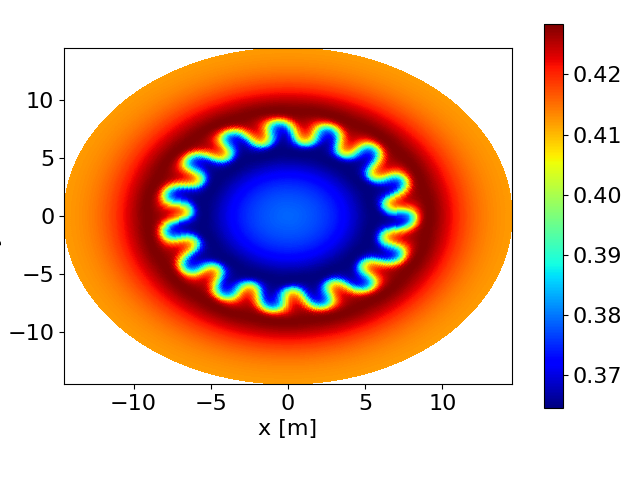
\includegraphics[width=\textwidth]{Figs/SimResults/t4000}
  \caption{T=4000}
 \end{subfigure}
 \begin{subfigure}[t]{.5\textwidth}
  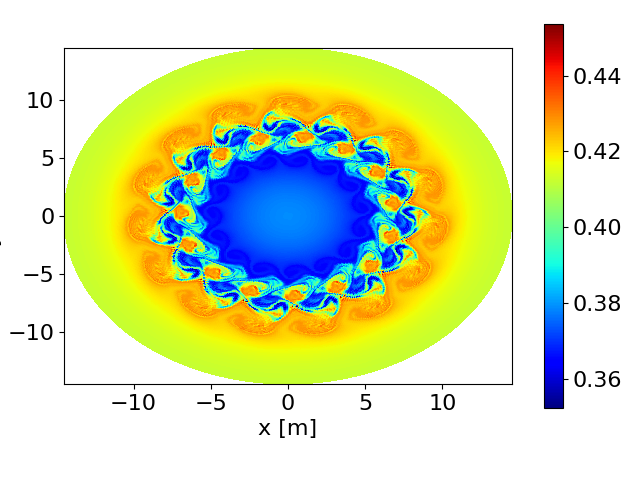
\includegraphics[width=\textwidth]{Figs/SimResults/t6000}
  \caption{T=6000}
 \end{subfigure}
 \caption{\label{fig::poloidal slice} Poloidal cut of the distribution function at different times at z=0 and $v_\parallel\approx0$}
\end{figure}

The equilibrium function as well as the radial profiles \{$T_i$ , $T_e$ , $n_0$ \} are defined in the paper by Latu et al. \cite{YamanPaper}.

The simulation results can be seen in figure \ref{fig::poloidal slice}. 


In addition to the poloidal slice the time evolution of the discrete L$^2$-norm of the electric potential is used as a diagnostic quantity. This norm is defined as follows:
\begin{equation}
 \left|\phi\right|_2(t):=\sqrt{\int_{r=r_{\min}}^{r=r_{\max}}\int_{\theta=0}^{\theta=2\pi}\int_{z=0}^{z=2\pi R_0}\phi(t,r,\theta,z)^2r\, dr\, d\theta\, dz}
\end{equation}

A trapezoidal rule is used to approximate the value. The results can be seen in figure \ref{fig::l2 phi}.

\begin{figure}
 \centering
 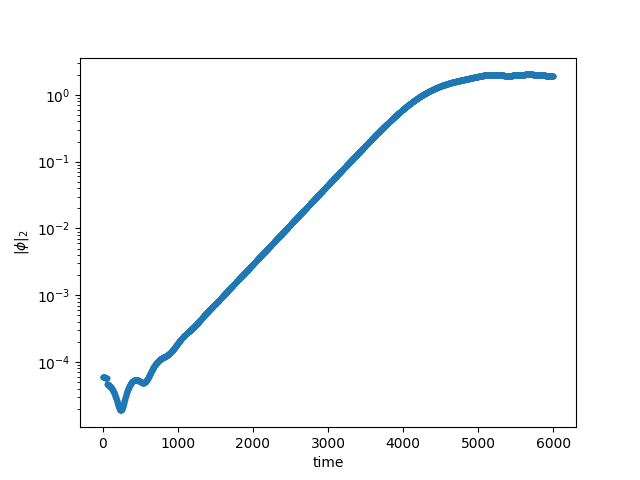
\includegraphics[width=.7\textwidth]{Figs/SimResults/l2}
 \caption{\label{fig::l2 phi}The time evolution of the discrete L$^2$-norm of the electric potential}
\end{figure}

We see that the L$^2$ norm demonstrates a linear phase as expected.
Unfortunately the gradient seen in this region is not what is expected. In addition while the poloidal planes demonstrate a similar shape to those seen by Latu et al. there appears to be some missing turbulence. We therefore conclude that the code still requires some debugging. Unfortunately time restrictions did not allow this step to be completed in time. The results so far are however close enough to the expected result to imply that it is possible to generate an accurate scientific code using this method.
% The gradient observed is in accordance with the dispersion relation as was the case for Latu et al. \cite{YamanPaper}. In addition the poloidal planes closely resemble those presented in their results. We therefore conclude that this code functions as expected and generates valid scientific results.




\rchapter{Conclusion}

%\bibliographystyle{IEEEtran}
% argument is your BibTeX string definitions and bibliography database(s)
\bibliographystyle{IEEEtran}
\bibliography{Thesis}{}
%\addcontentsline{toc}{chapter}{\refname}

\end{document}
